% ff5-tutorial-guide.tex
% PJ, 02-aug-2012 ff 3.8
% PJ, 26-Apr-2014 ff 5.0
%     19-Jan-2016 ff 5.0 update to new processors

\documentclass[12pt,a4paper]{article}
\usepackage[body={16cm,24cm}]{geometry}
\usepackage{hyperref}
\hypersetup{colorlinks=true,linkcolor=blue}
\usepackage{graphicx}
% \usepackage{bytefield}
\usepackage{listings}
\pagestyle{headings}

\lstset{basicstyle=\ttfamily, showstringspaces=false, identifierstyle=, keywordstyle=}
\lstset{numbers=left, numberstyle=\tiny, stepnumber=1, numbersep=5pt}
\newcommand{\code}[2]{
 \hrulefill
 \scriptsize
 \lstinputlisting{#2}
 \hrulefill
 \vspace{2em}
 \normalsize
}

%------------------------------------------------------------------
% a couple horizontal bars to delimit embedded code
% the width suits that set above and
% the mathmode eliminates spaces between the three elements
\newcommand{\topbar}{\ensuremath{
    \rule{0.1mm}{2.0mm} \rule[2.0mm]{159.5mm}{0.1mm} \rule{0.1mm}{2.0mm}
}}
\newcommand{\bottombar}{\ensuremath{
    \rule{0.1mm}{2.0mm} \rule{159.5mm}{0.1mm} \rule{0.1mm}{2.0mm}
}}

%------------------------------------------------------------------

\title{
    A Tutorial Guide to Programming PIC18, PIC24 \\
    and ATmega Microcontrollers with FlashForth. \\
    2016 Revision
}
\author{
    Mechanical Engineering Report 2016/01\\
    P. A. Jacobs\\
    School of Mechanical and Mining Engineering\\
    The University of Queensland.
}
%\date{January, 2016}

\begin{document}
\maketitle

\centerline{\textbf{Abstract}}
\medskip\noindent
Modern microcontrollers provide an amazingly diverse selection of hardware
peripherals, all within a single chip.
One needs to provide a small amount of supporting hardware to power the chip
and connect its peripheral devices to the signals of interest and, when powered up,
these devices need to be configured and monitored by a suitable firmware program.

\medskip\noindent
These notes focus on programming the 28-pin PIC18F26K22 microcontroller and
its 40-pin PIC18F46K22 sibling, 
the 16-bit PIC24FV32KA302 and 
the 8-bit AVR ATmega328P.
These microcontrollers are all available in plastic DIP packages, 
can be run from a 5 volt supply,
and can be built into very simple prototype hardware.

\medskip\noindent
A number of example programs, in the Forth language, are provided 
to illustrate the use of some of each microcontroller's peripheral devices.
The examples cover the very simple ``flash a LED'' exercise through to driving
a character-based LCD via its 4-bit parallel interface.
Communication with SPI and I$^2$C devices is also covered, with a common set of words
being used to abstract away the differences between microcontrollers 
in terms of detailed bits and registers.


\newpage
\tableofcontents

\newpage
\section{A selection of microcontrollers}
%
Over the past couple of decades, microcontrollers have evolved to be
cheap, powerful computing devices that even Mechanical Engineers can 
use in building bespoke instrumentation for their research laboratories.
Typical tasks include monitoring of analog signals, sensing pulses and 
providing timing signals.
Of course these things could be done with a modern personal computer
connected via USB to a commercial data acquisition and signal processing system
but there are many situations where the small, dedicated microcontroller,
requiring just a few milliamps of current, performs the task admirably 
and at low cost.

\medskip\noindent
Modern microcontrollers provide an amazingly diverse selection of hardware
peripherals, all within a single chip.
One needs to provide a small amount of supporting hardware to power the chip
and connect its peripheral devices to the signals of interest and, when powered up,
these devices need to be configured and monitored by a suitable firmware program.
These following sections provide an introduction to the details of doing this 
with an 8-bit Microchip PIC18F26K22 or PIC18F46K22 microcontroller, 
a 16-bit Microchip PIC24FV32KA302 microcontroller
and an 8-bit Atmel ATmega328P microcontroller, 
all programmed with the FlashForth version 5 interpreter\,\cite{nordman_2014a}.

\medskip\noindent
Within each family of Microchip or Atmel microcontrollers, 
the individual microcontroller units (MCUs) all have the same core, 
\emph{i.e.} same instruction set and memory organisation.
Your selection of which MCU to actually use in your project can be based on
a couple of considerations.
If you are on a tight budget and will be making many units, 
choose an MCU with just enough functionality, however,
if convenience of development is more important, 
choose one with ``bells and whistles''. 
For this tutorial guide, we will value convenience and so 
will work with microcontrollers that have:
\begin{itemize}
  \item a nice selection of features, including a serial port, 
     several timers and an analog-to-digital converter.
     See the feature list and the block diagram of the PIC18F26K22 and 
     PIC18F46K22 MCUs on the following pages.
  \item a 28-pin narrow or 40-pin DIL package, which is convenient for prototyping and
     has enough I/O pins to play without needing very careful planning.
  \item an ability to work as 3.3V or 5V systems.
  \item a pinout as shown at the start of the datasheets 
     (books)\,\cite{pic18f26k22-datasheet,pic24fv32ka302-datasheet,atmega328-datasheet}.
     You will be reading the pages of these books over and over but we include 
     the following couple of pages from the PIC18F22K26/PIC18F46K22 datasheet to give an overview.
  \item an internal arrangement that is built around an 8-bit or 16-bit data bus.
  \item the ``Harvard architecture'' with separate paths and storage areas for program 
     instructions and data.
\end{itemize}
We won't worry too much about the details of the general-purpose registers,
the internal static RAM or the machine instruction set because we will let
the FlashForth interpreter handle most of the details, however, 
memory layout, especially the I/O memory layout is important for us as programmers.
The peripheral devices, which are used to inferface with the real world,
are controlled and accessed via registers in the data-memory space.

\newpage
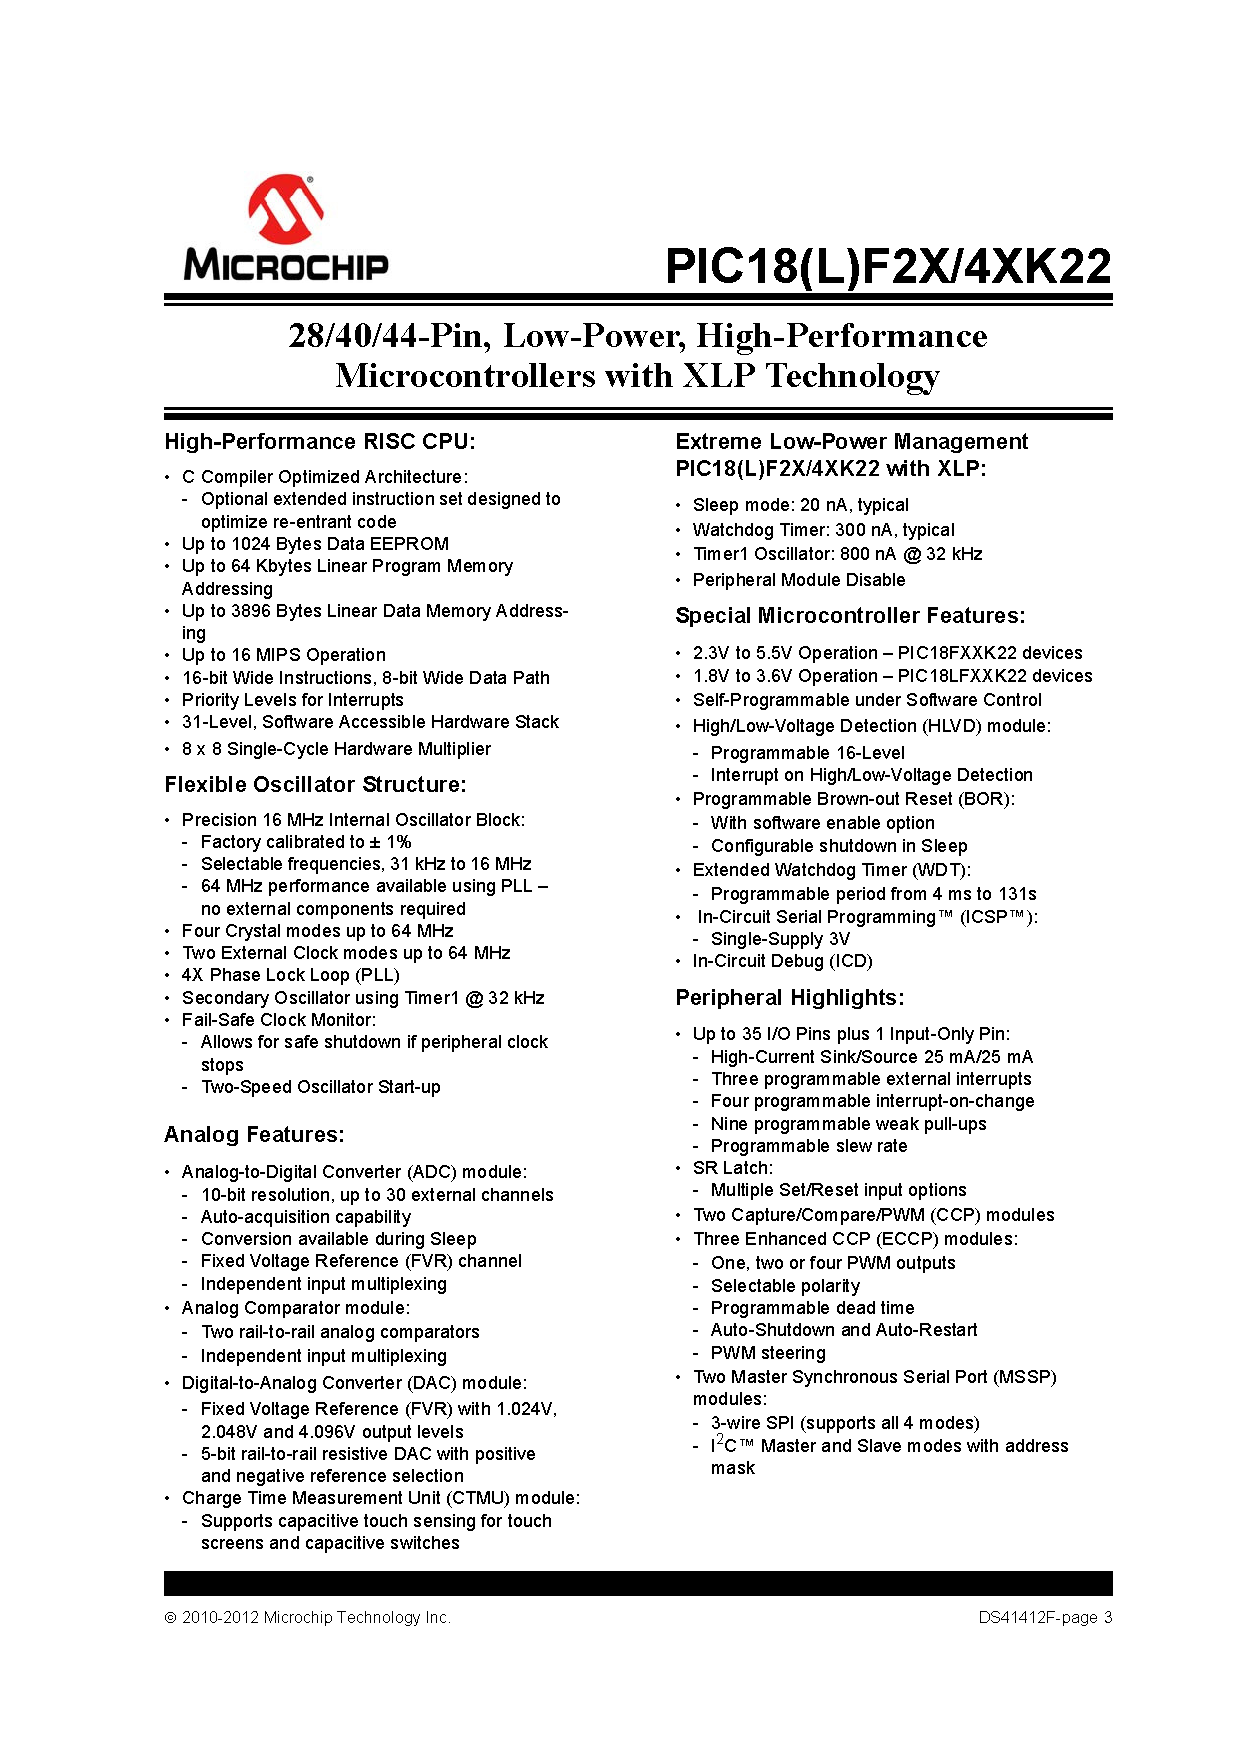
\includegraphics[width=0.95\textwidth,viewport=73 56 545 772,clip=true]{../figs/pic18f26k22-features-from-datasheet.pdf}

\newpage
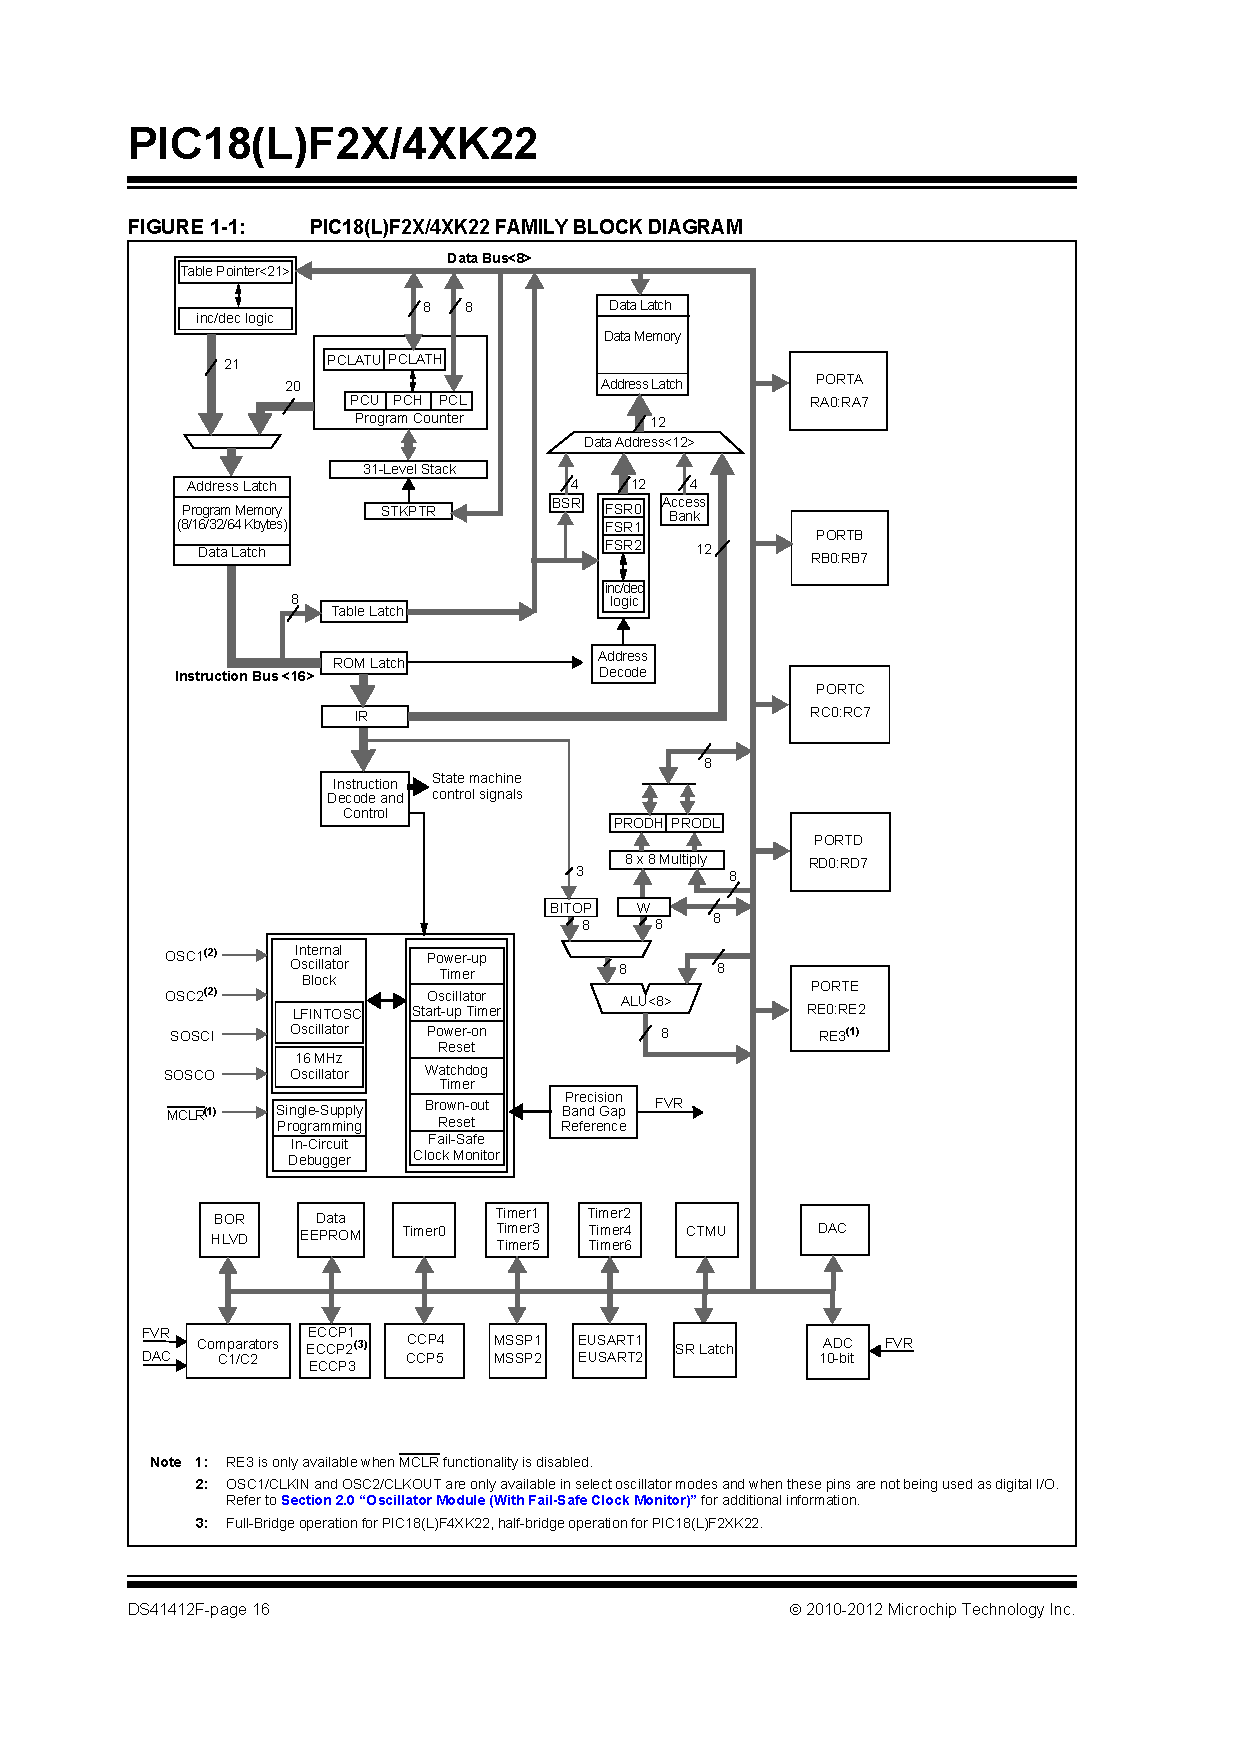
\includegraphics[width=0.95\textwidth,viewport=57 64 518 781,clip=true]{../figs/pic18f26k22-block-diagram-from-datasheet.pdf}

 
\newpage
\section{Development boards}
%
This tutorial is based around simple support hardware for each of the microcontrollers.
If you don't want to do your own soldering, there are easy-to-buy demonstration boards 
available as a convenient way to get your hardware up and going.
If you are a student of mechatroncis, however, you must eventually design and build your own hardware.  
The strip-board versions are aimed at you.

\medskip
\subsection{PIC18 family boards}
%
Here is a picture of PICDEM 2 PLUS with PIC18F46K22-I/P in the 40-pin socket (U1)
and running the LCD, as described in Section\,\ref{lcd-example-sec}.
We'll make use of the serial RS-232 interface (MAX232ACPA, U3) to both program Forth application and 
to communicate with running applications.
Other conveniences include on-board LEDs, switches, a potentiometer (RA0) 
and I$^2$C devices, such as a TC74 temperature sensor (U5), just below the MCU
and a 24LC256 serial EEPROM (U4).
Initial programming of the FlashForth system into the MCU can be done via jack J5 
(labelled ICD in the lower left of the photograph)
with a Microchip MPLAB-ICD3, PICkit3, or similar device programmer.

\bigskip
\noindent
{
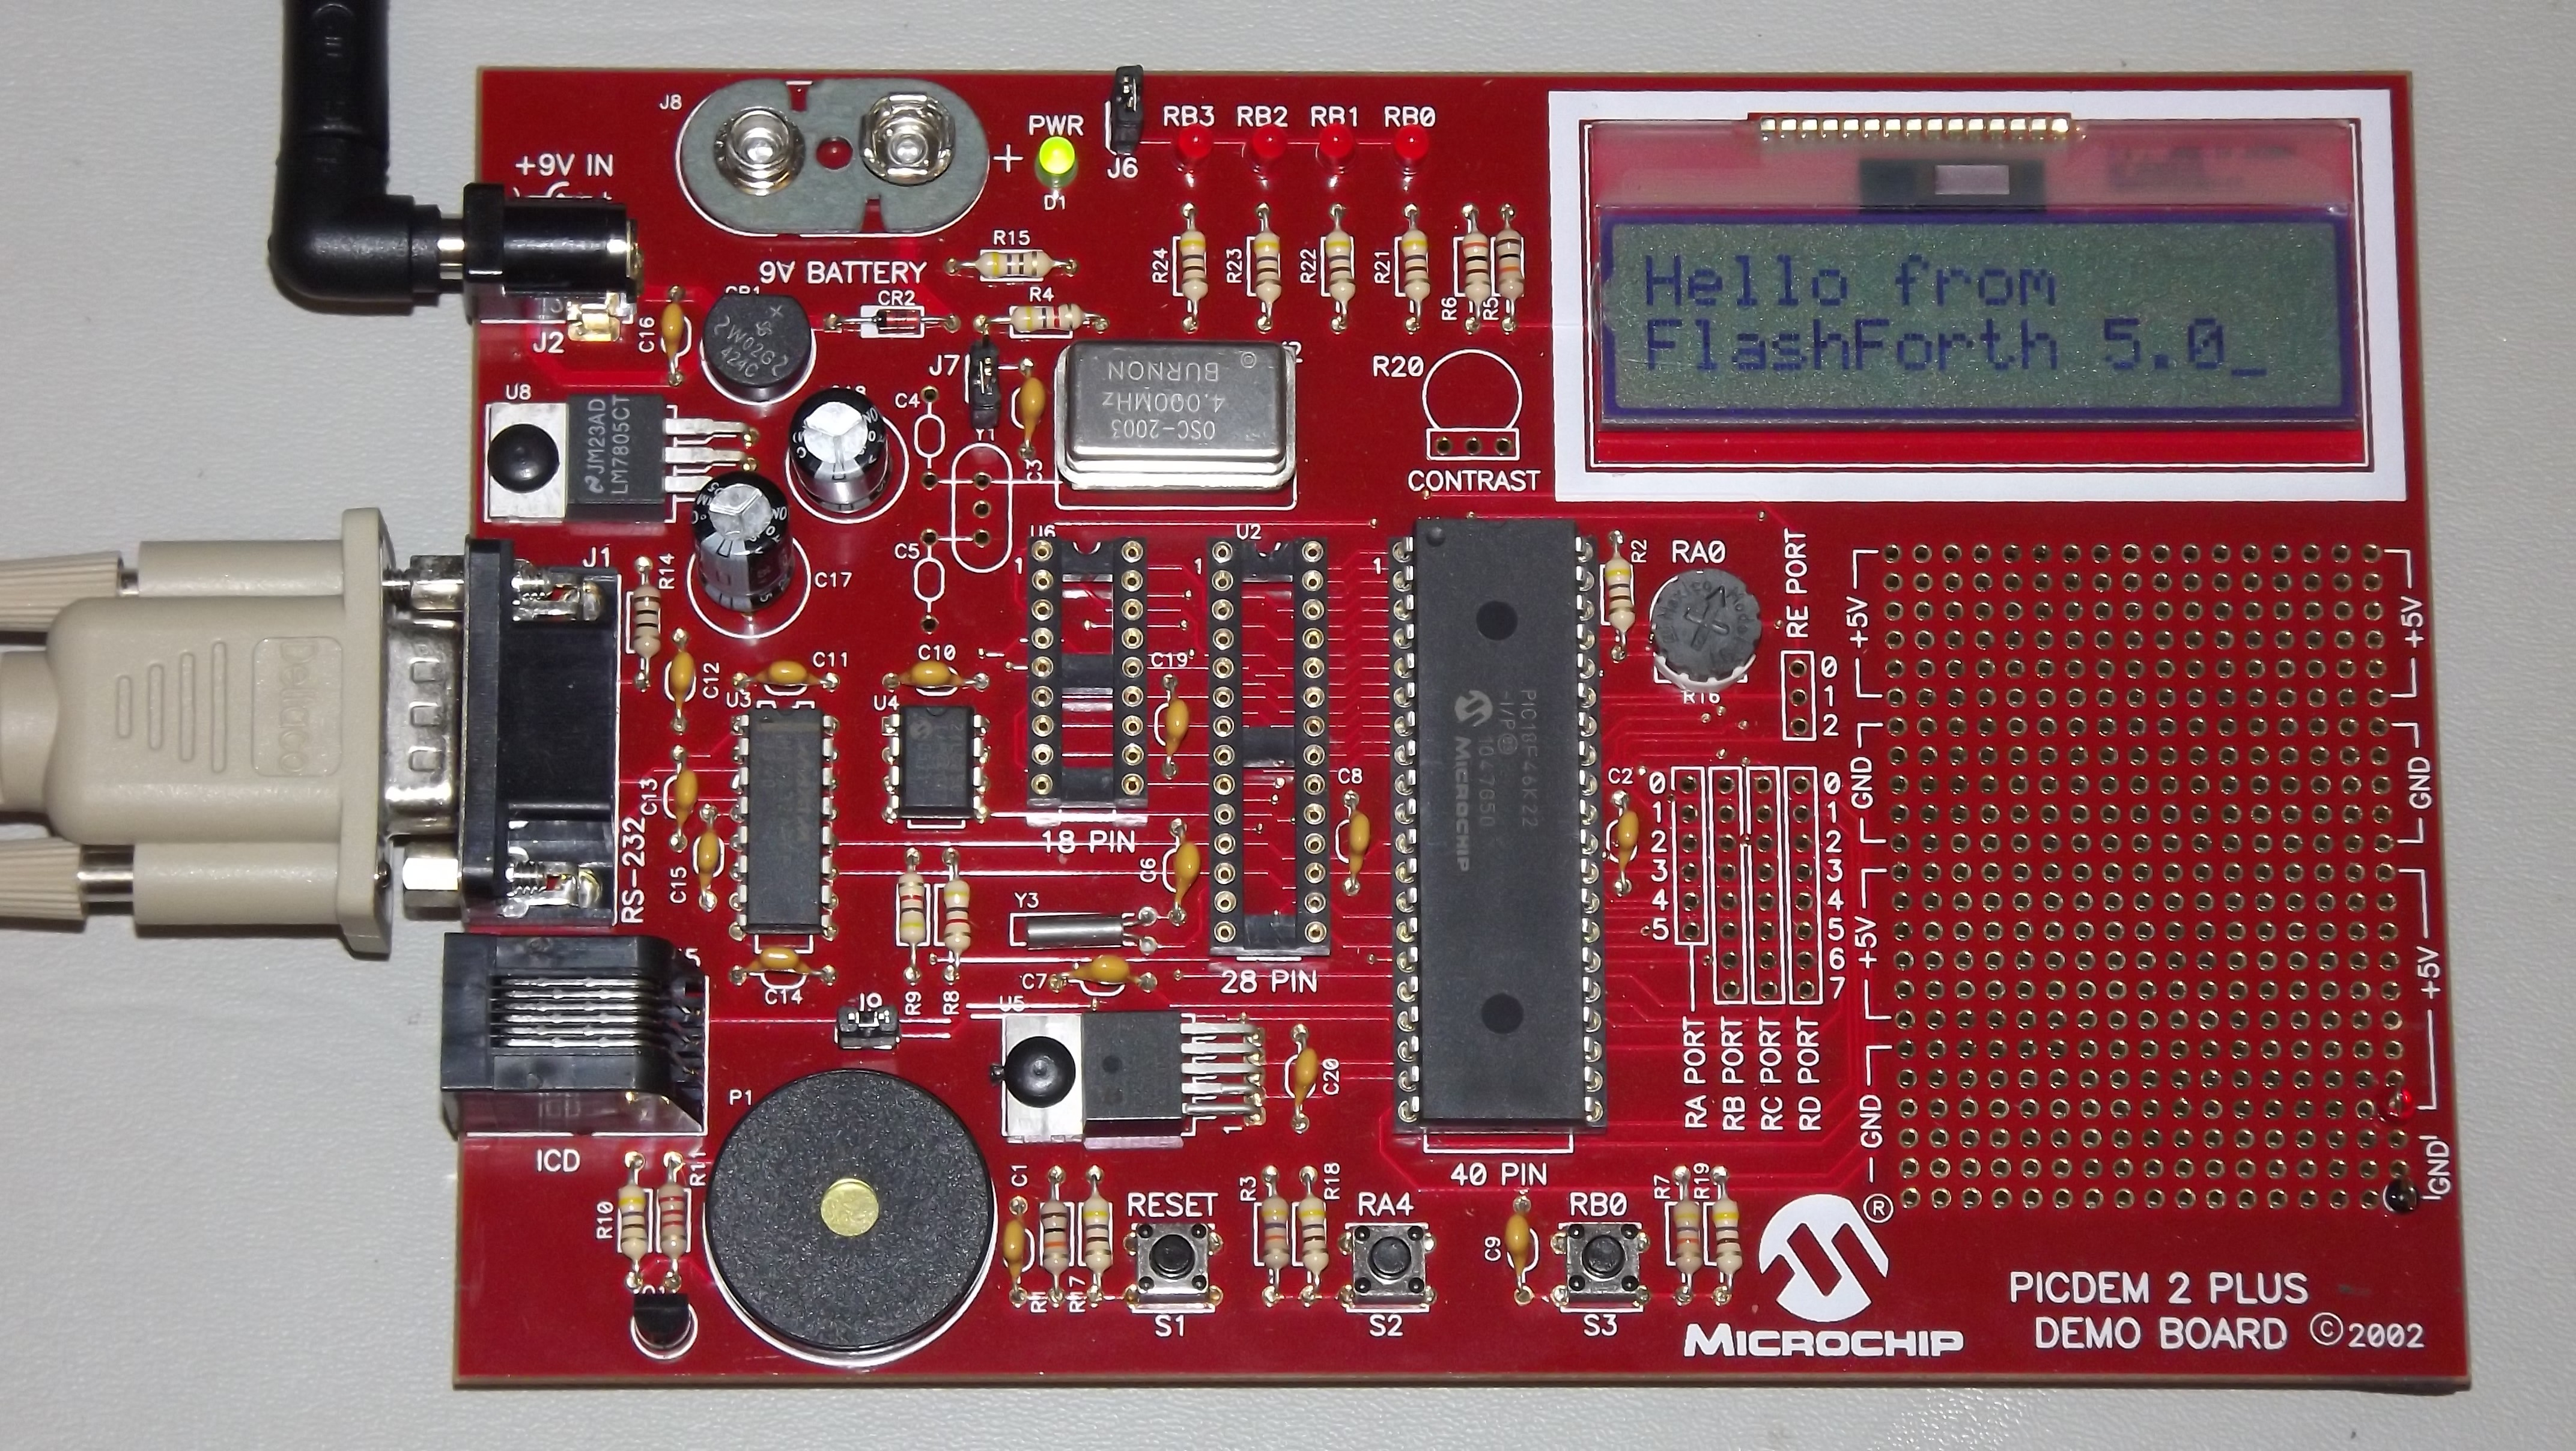
\includegraphics[width=0.95\textwidth]{../figs/picdem2plus-with-46k22-flashforth-5.jpeg}
\label{lcd-on-picdem2-board}
}

\bigskip\noindent
If you want a homebrew system, 
you can build a minimal system on strip-board that works well.
One of the nice things about such a strip-board construction is that you can
easily continue construction of your bespoke project on the board and,
with careful construction, your prototype can provide years of reliable service. 

\medskip
\centerline{
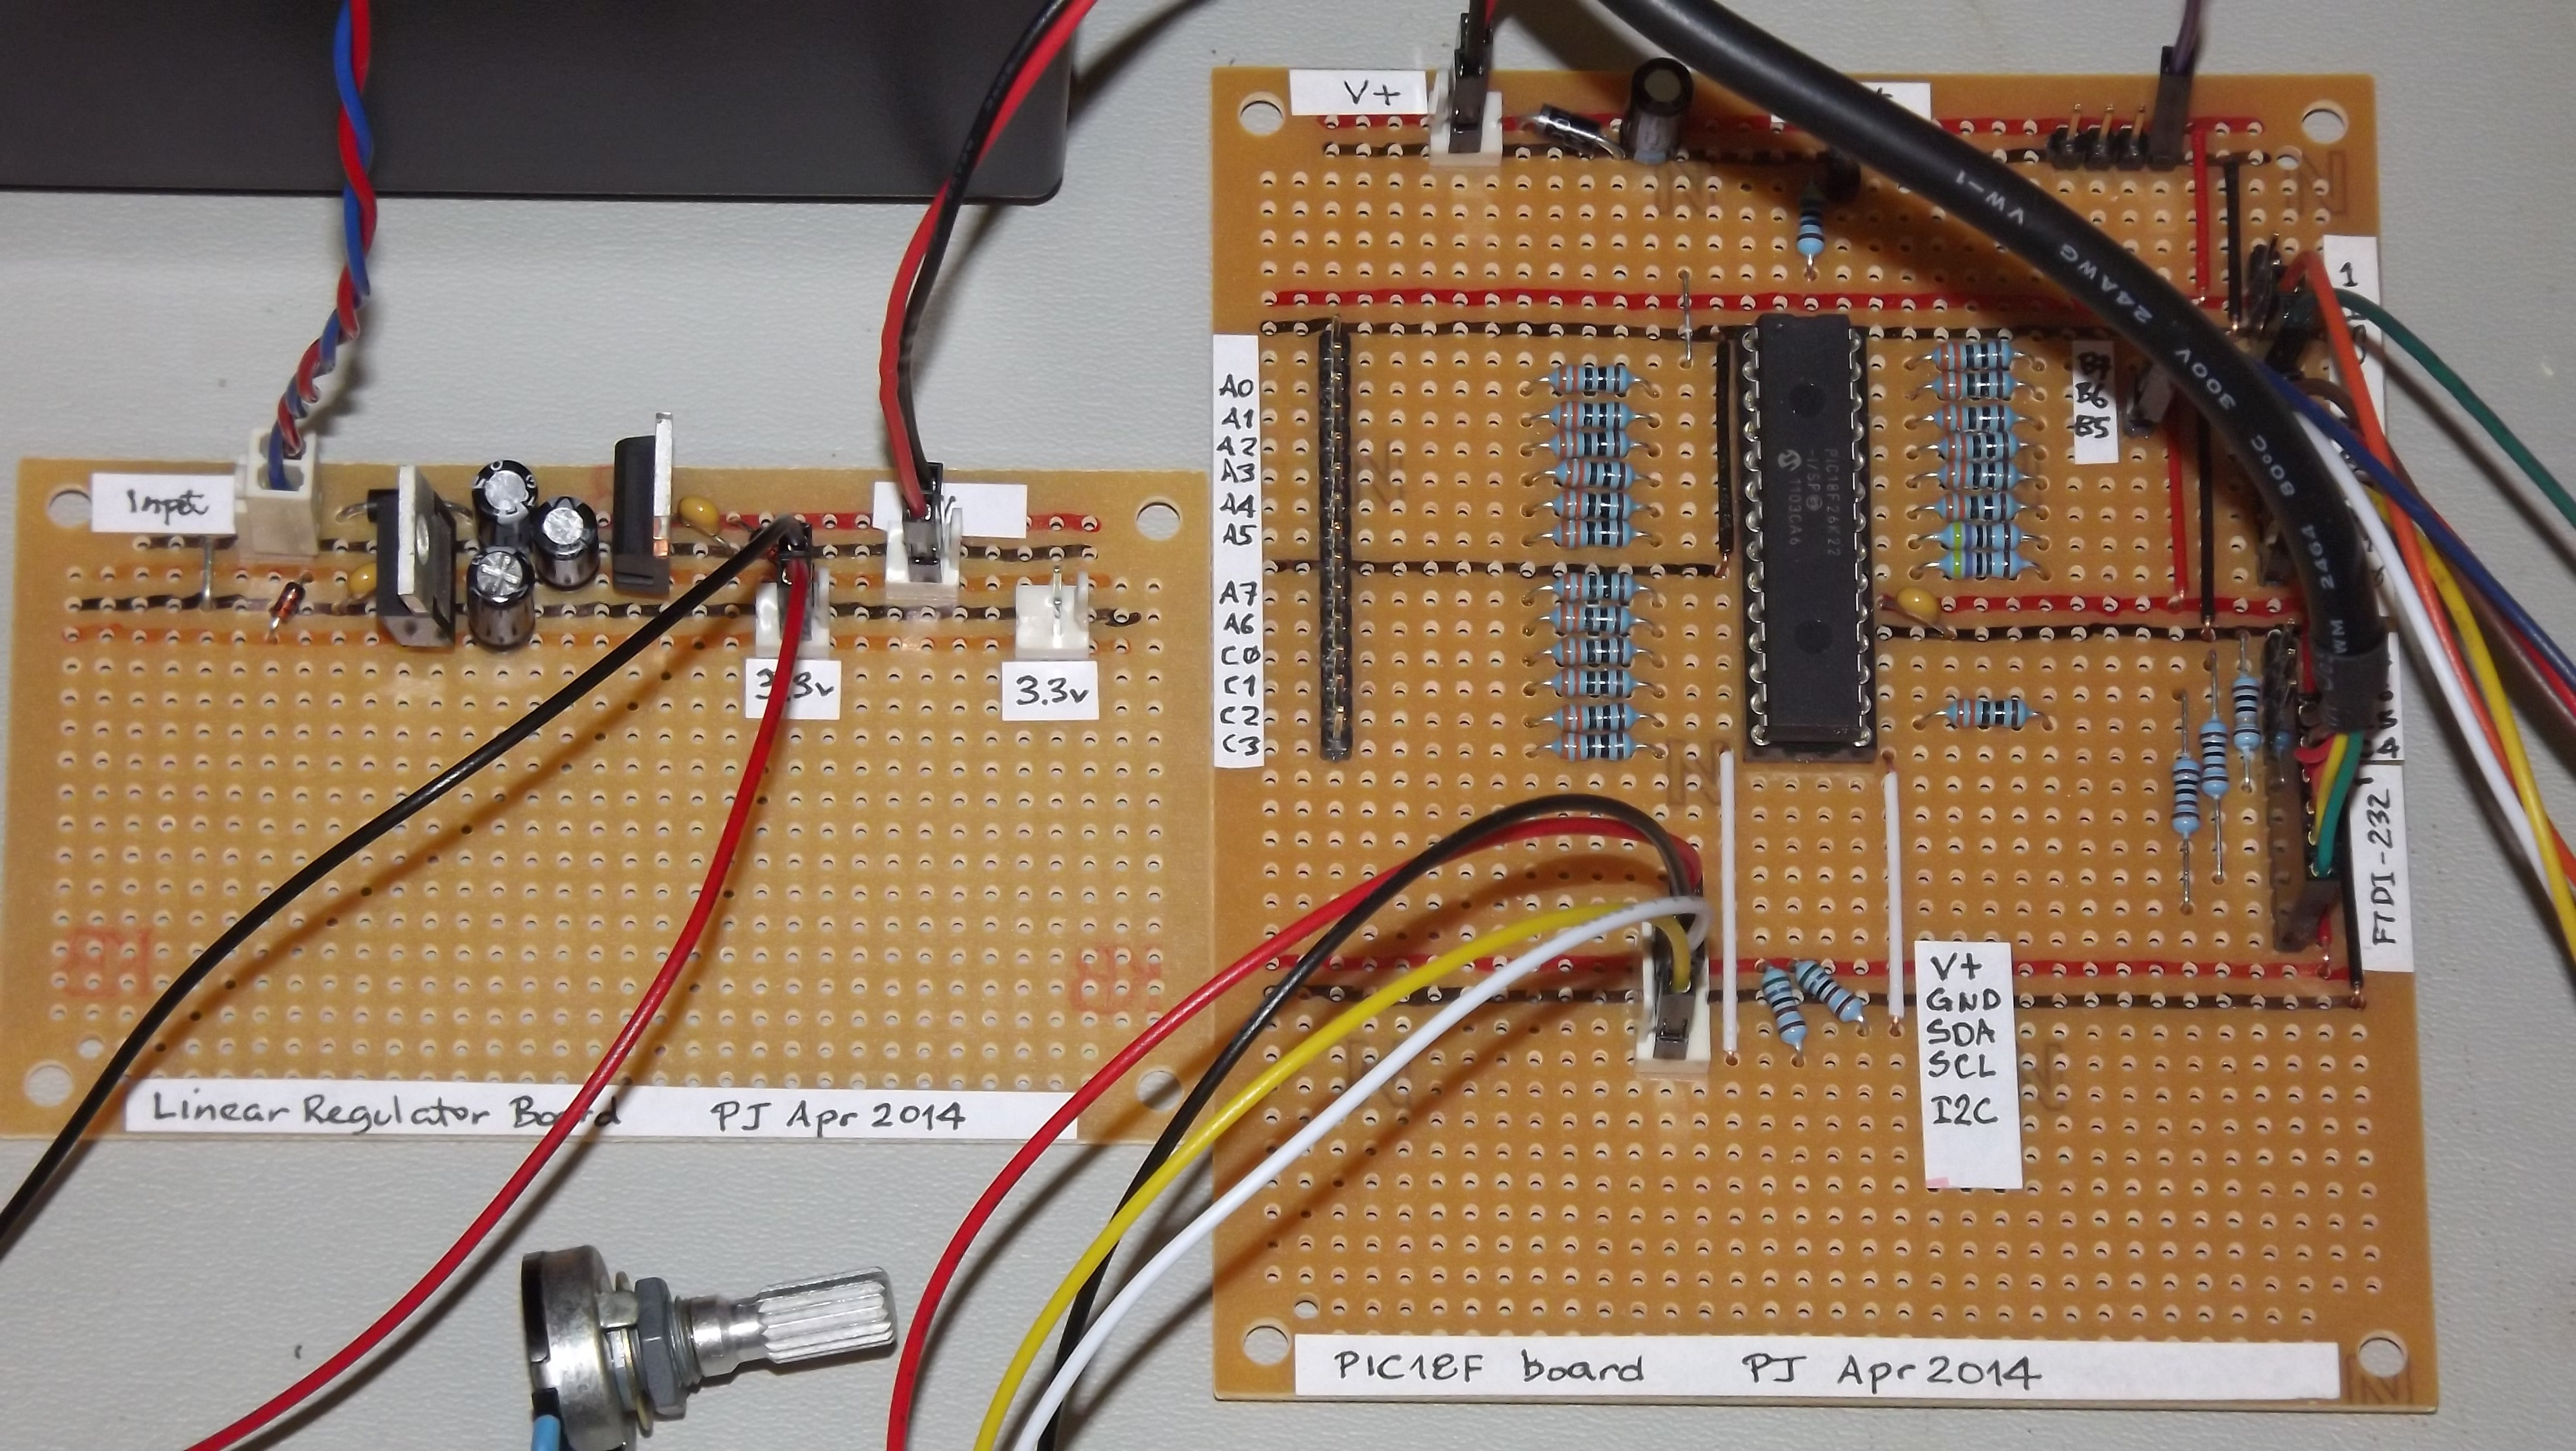
\includegraphics[width=0.9\textwidth]{../figs/pic18f26k22-demo-board-with-regulator-board-2014.jpeg}
}

\medskip\noindent
Here is a detailed view of the home-made demo board with PIC18F26K22 in place.
This board is suitable for the exercises in this guide.
A separate regulator board is to the left and a current-limited supply provides the 
input power.
The board is simple to make by hand, with header pins for the reset switch and connections to the LEDs.
The 4-pin header in the foreground provides an I$^2$C connection.
The ICSP header is only needed to program FlashForth into the MCU, initially.
All communication with the host PC is then via the TTL-level serial header (labelled FTDI-232) at the right.
Beyond the minimum required to get the microcontroller to function, 
we have current-limiting resistors and header pins on most of the MCU's I/O pins.
This arrangement is convenient for exercises such as interfacing to the 4x3 matrix keypad
(Section\,\ref{4x3-keypad-section}).

\medskip\noindent
The schematic diagram of this home-brew board is shown on the following page.
Note that there is no crystal oscillator on the board; the internal oscillator is 
sufficiently accurate for asynchronous serial port communication.
Note, also, the 1k resistors in the TX and RX nets.  
These limit the current going through the microcontroller pin-protection diodes
in the situation where the microcontroller board is unpowered and the FTDI-232 cable
is still plugged in to your PC.
This will happen at some point and, without the current-limiting resistors, the FTDI cable
will power the microcontroller, probably poorly.


\newpage
\noindent
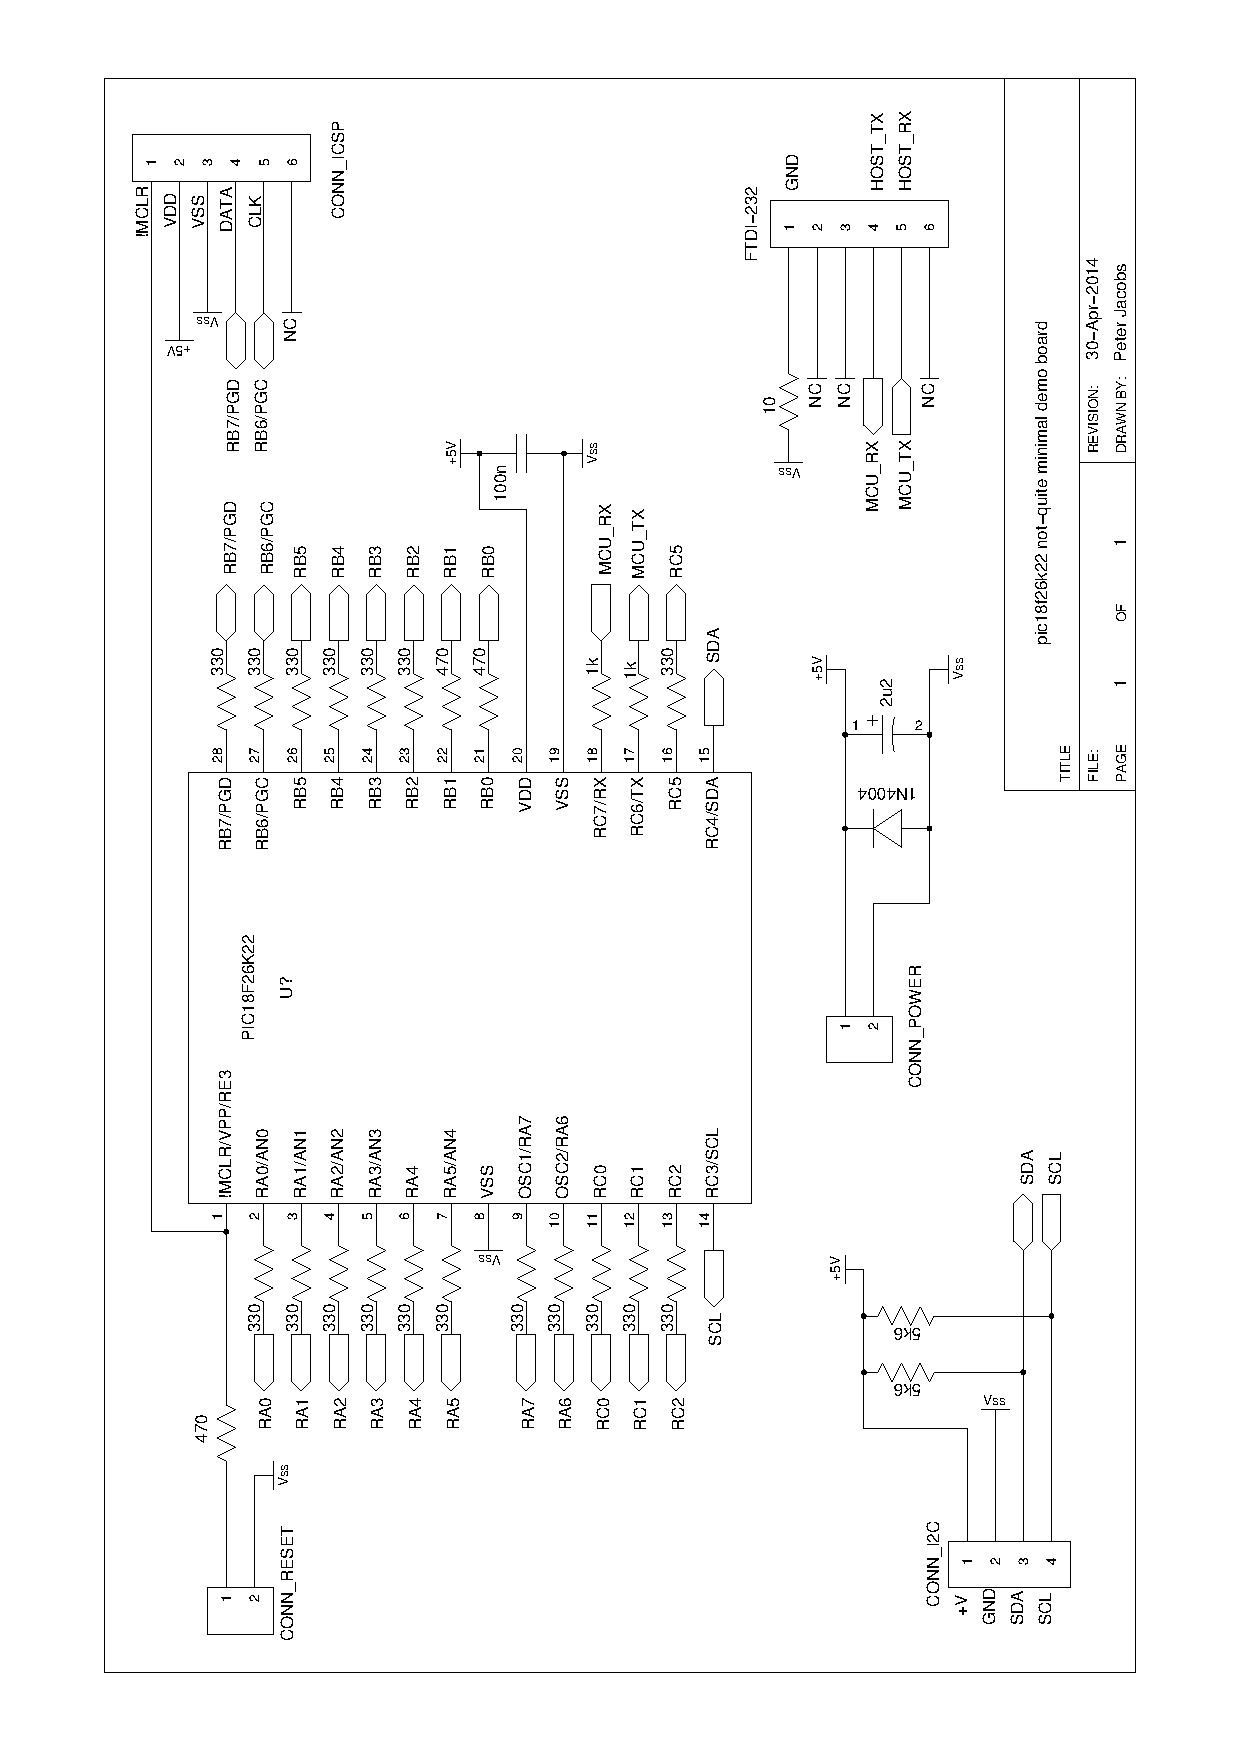
\includegraphics[width=\textwidth,angle=0,viewport=48 37 547 806]{../figs/demo-board-schematic-26k22.pdf}

\medskip
\subsection{AVR and PIC24 boards}
%
The Eleven from Freetronics, shown in the left half of the following photograph,
is an Arduino-compatible board carrying an ATmega328P microcontroller.
This is a convenient piece of hardware with many prototype-friendly boards 
available to plug into the headers around the periphery of the board.
Although these boards come with the Arduino bootloader preprogrammed into the 
ATmega328 microcontroller, the standard AVR 6-pin programming header on the
right-hand end of the board (in the photo) can be used to reprogram the microcontroller
with the FlashForth interpreter.
Power and serial port access is through the USB connector at the left.

\medskip\noindent
If you want an almost-no-solder option for prototyping with the PIC24FV32KA302, 
Microchip provide the Microstick 5V for PIC24K-series.
As shown in the following photograph, this is convenient in that it includes 
a programmer on-board and can be plugged into a bread-board.
The power supply and flash programming access is provided through the USB connector 
on the left of the board while the serial port connection is via the 6-pin connector 
on the right-end of the board.

\medskip
\centerline{
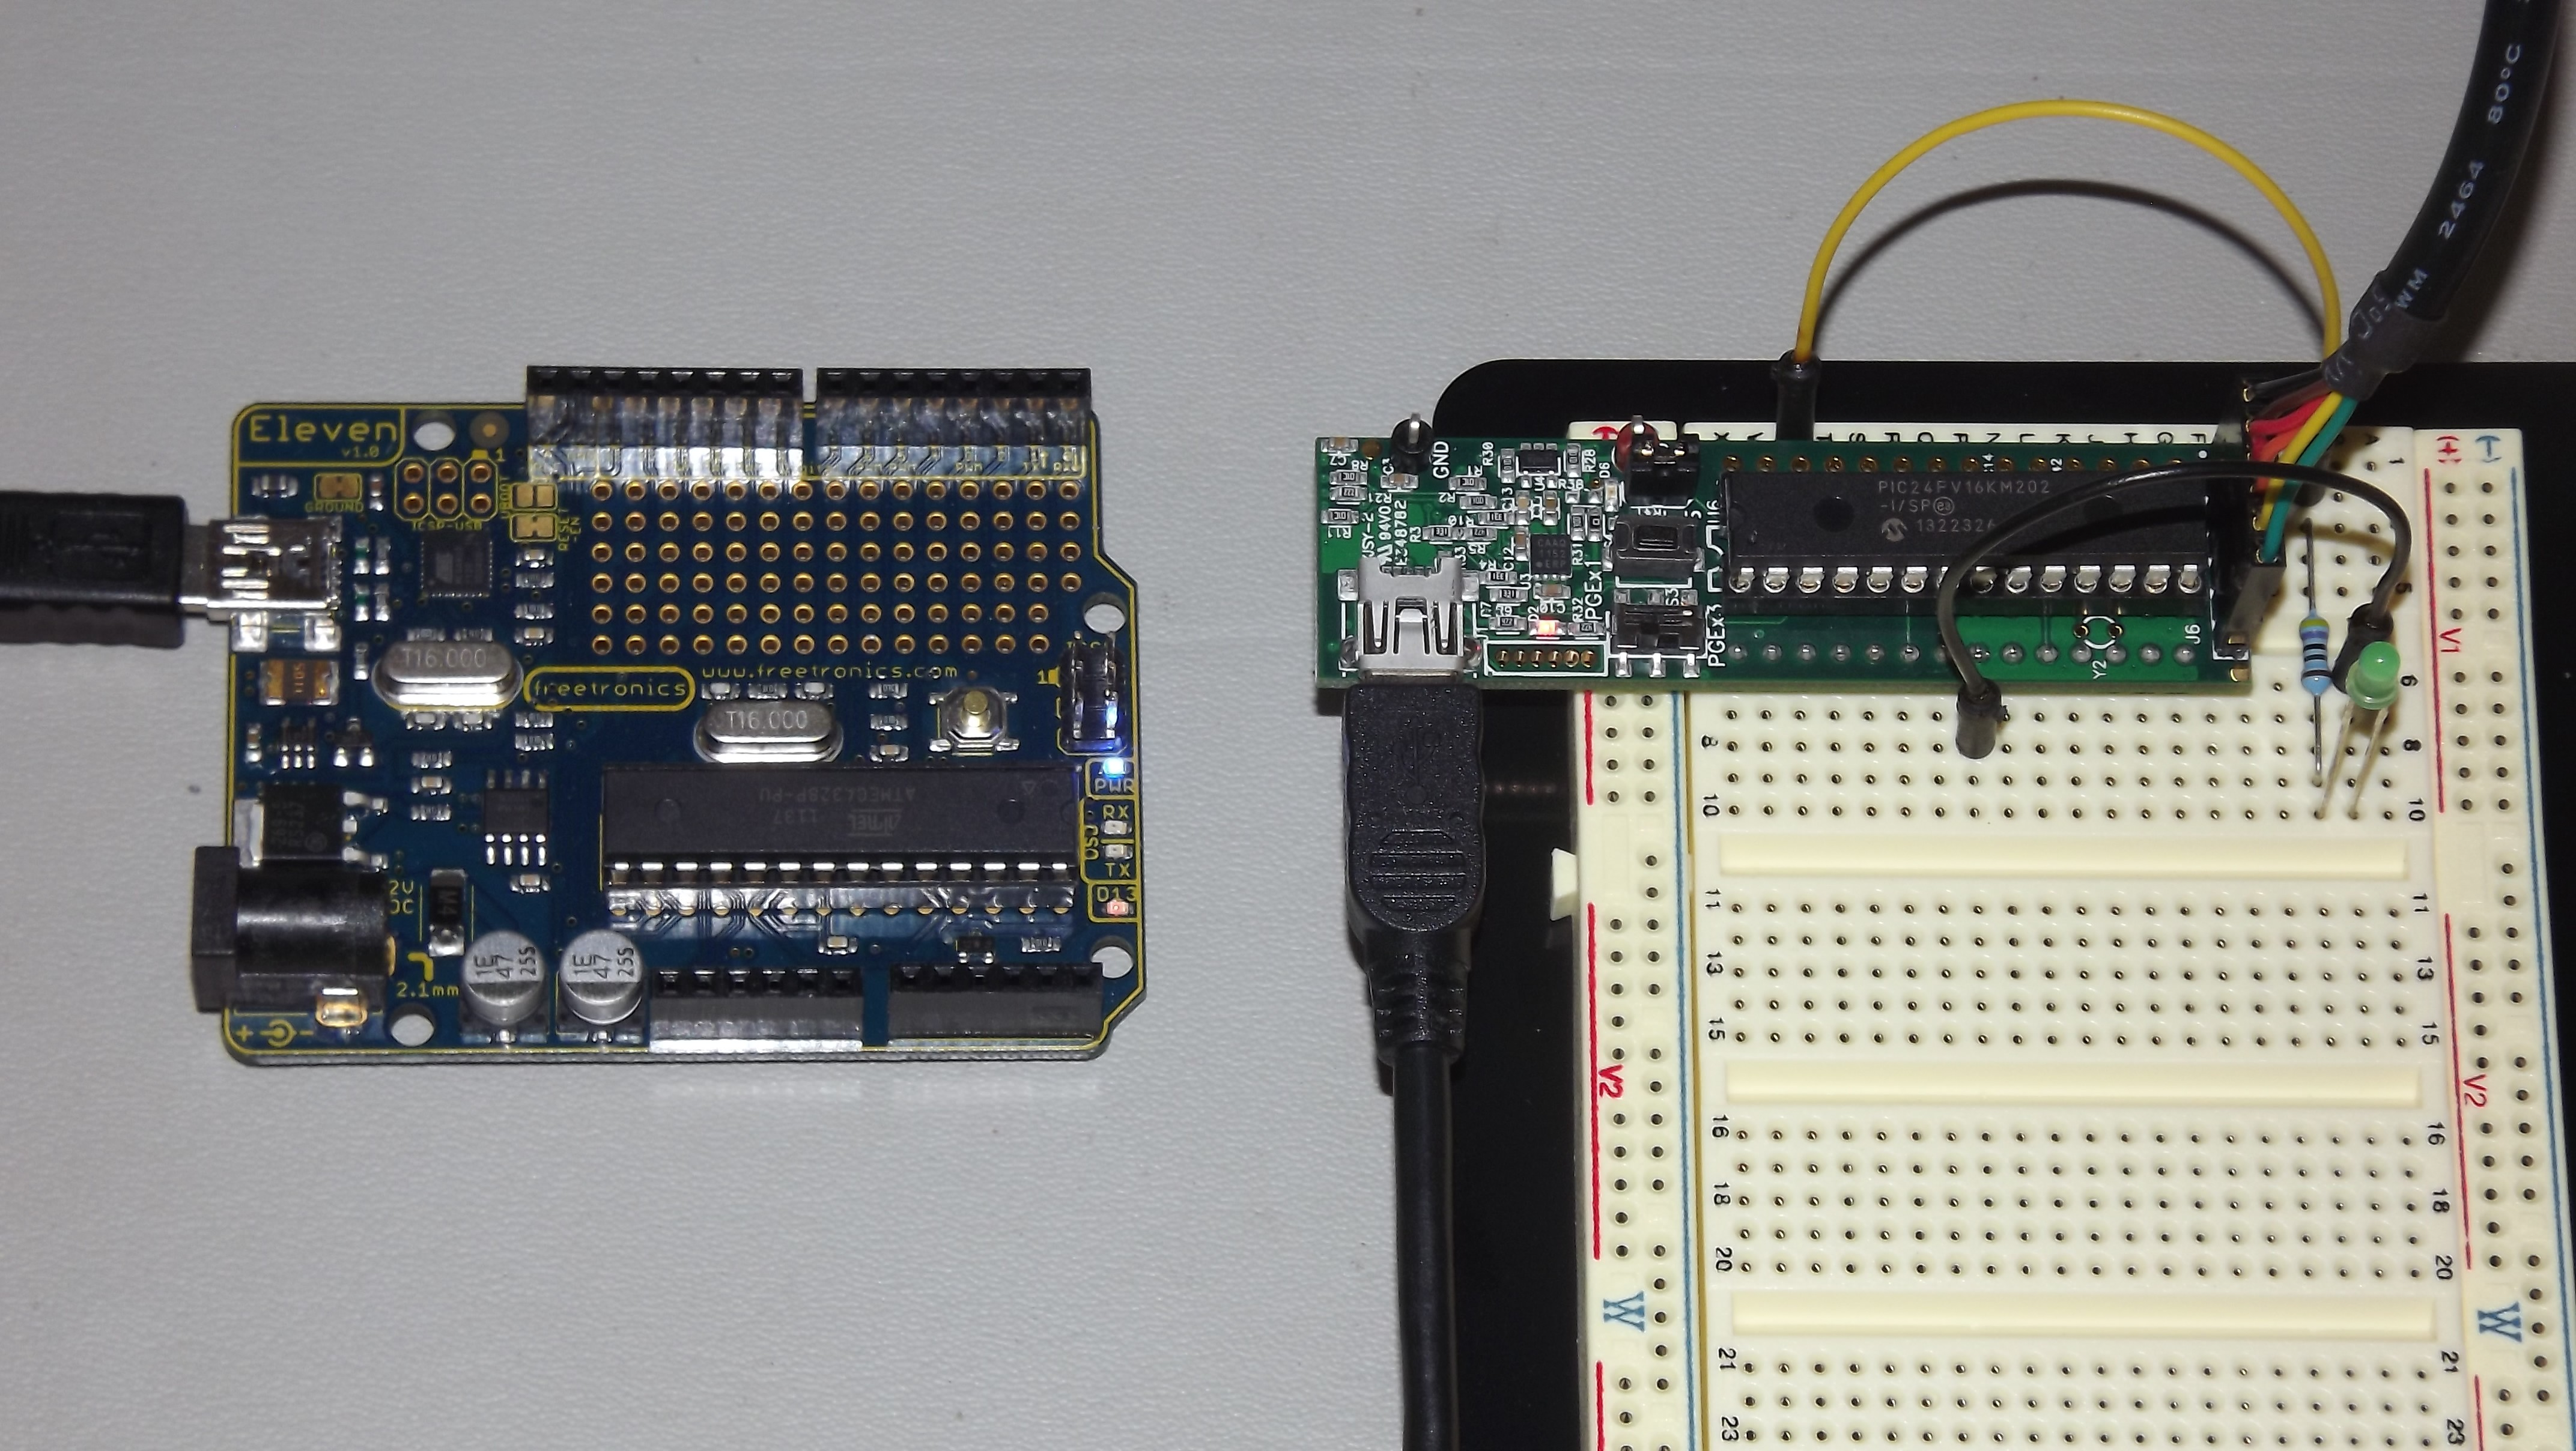
\includegraphics[width=0.9\textwidth]{../figs/eleven-and-microstick-boards-2014.jpeg}
}

\newpage
\noindent
Building a minimal board, by hand, for any of these processors is fairly easy and 
strip-board versions for each is shown in the following photograph.
The left-hand board is for the PIC18F26K22, before all of the extra protection resistors
were added.  In this state, FlashForth can already be used on this board for nearly all 
of the exercises in the following sections.
Schematic diagrams for the PIC24 and AVR microcontrollers are shown on the following pages.

\medskip
\centerline{
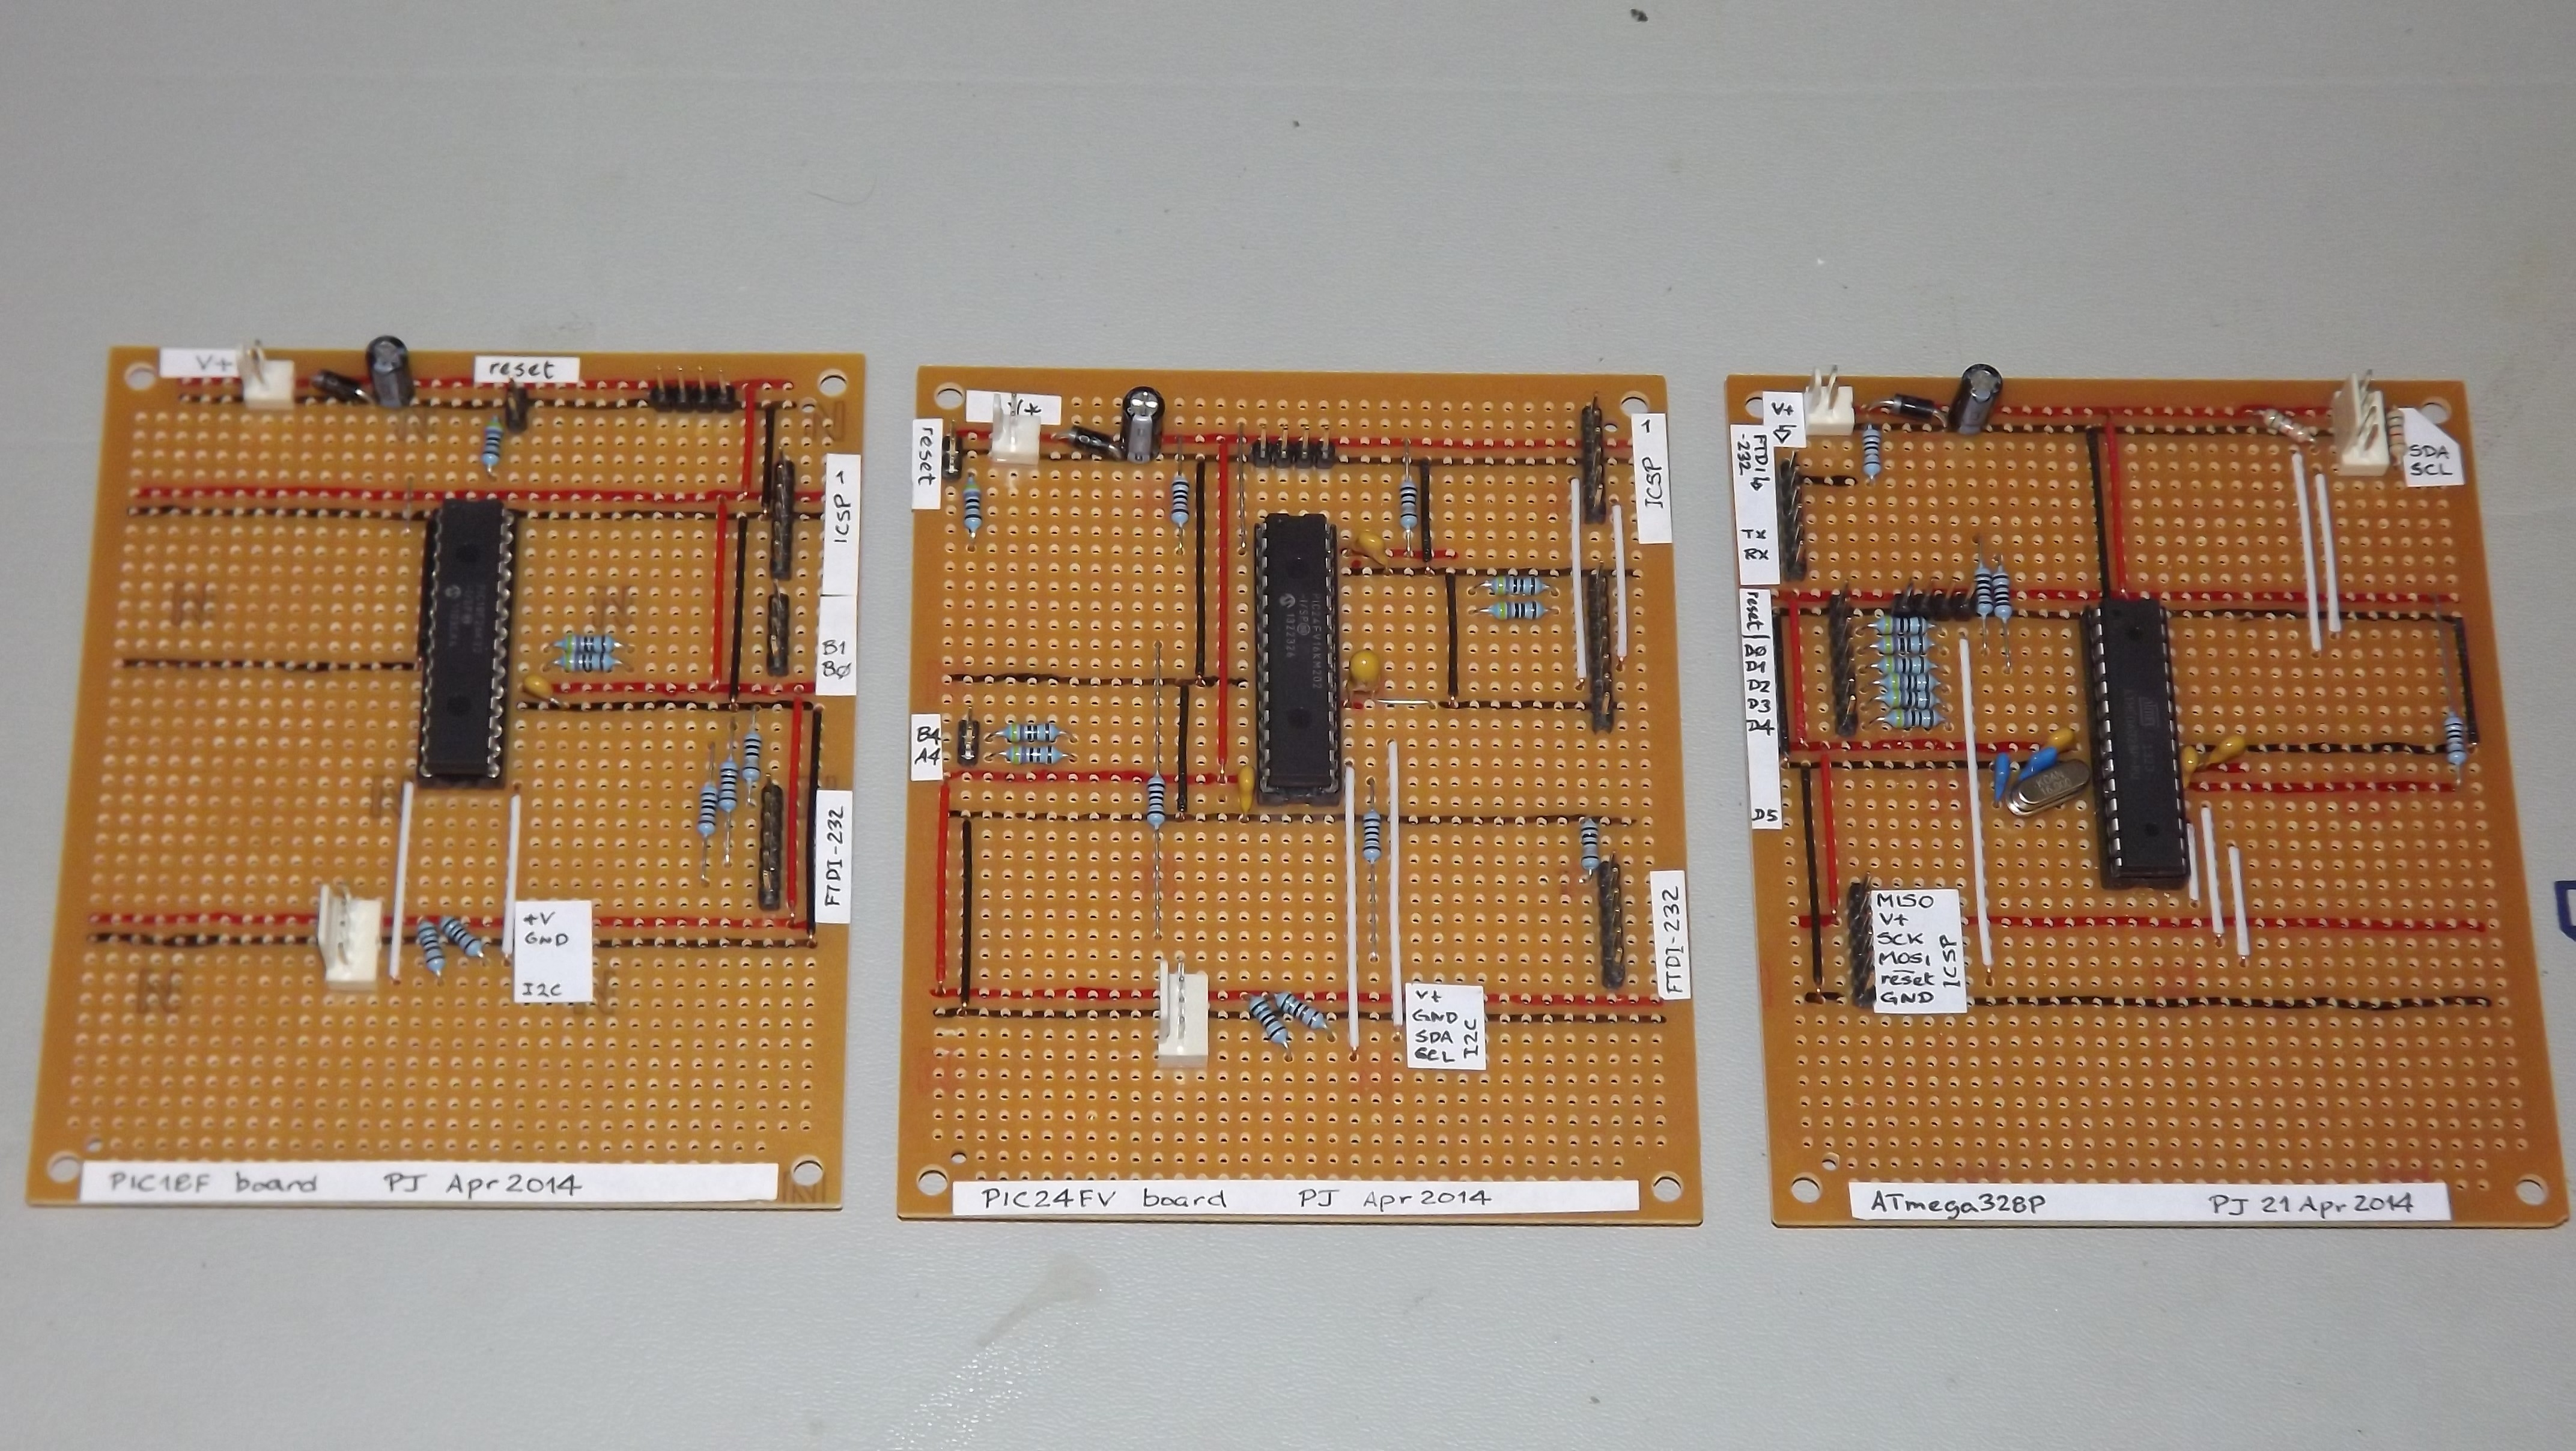
\includegraphics[width=0.9\textwidth]{../figs/home-built-minimal-boards-2014.jpeg}
}

\medskip\noindent
Each of the boards has headers for (1) power, (2) in-circuit serial programming, (3) I2C communication and
(4) TTL-level-232 serial communication.
The ATmega328 board on the right has a few more protection resistors installed and has
an 16\,MHz crystal because serial-port communication was found to be unreliable using the internal oscillator.

\newpage
\noindent
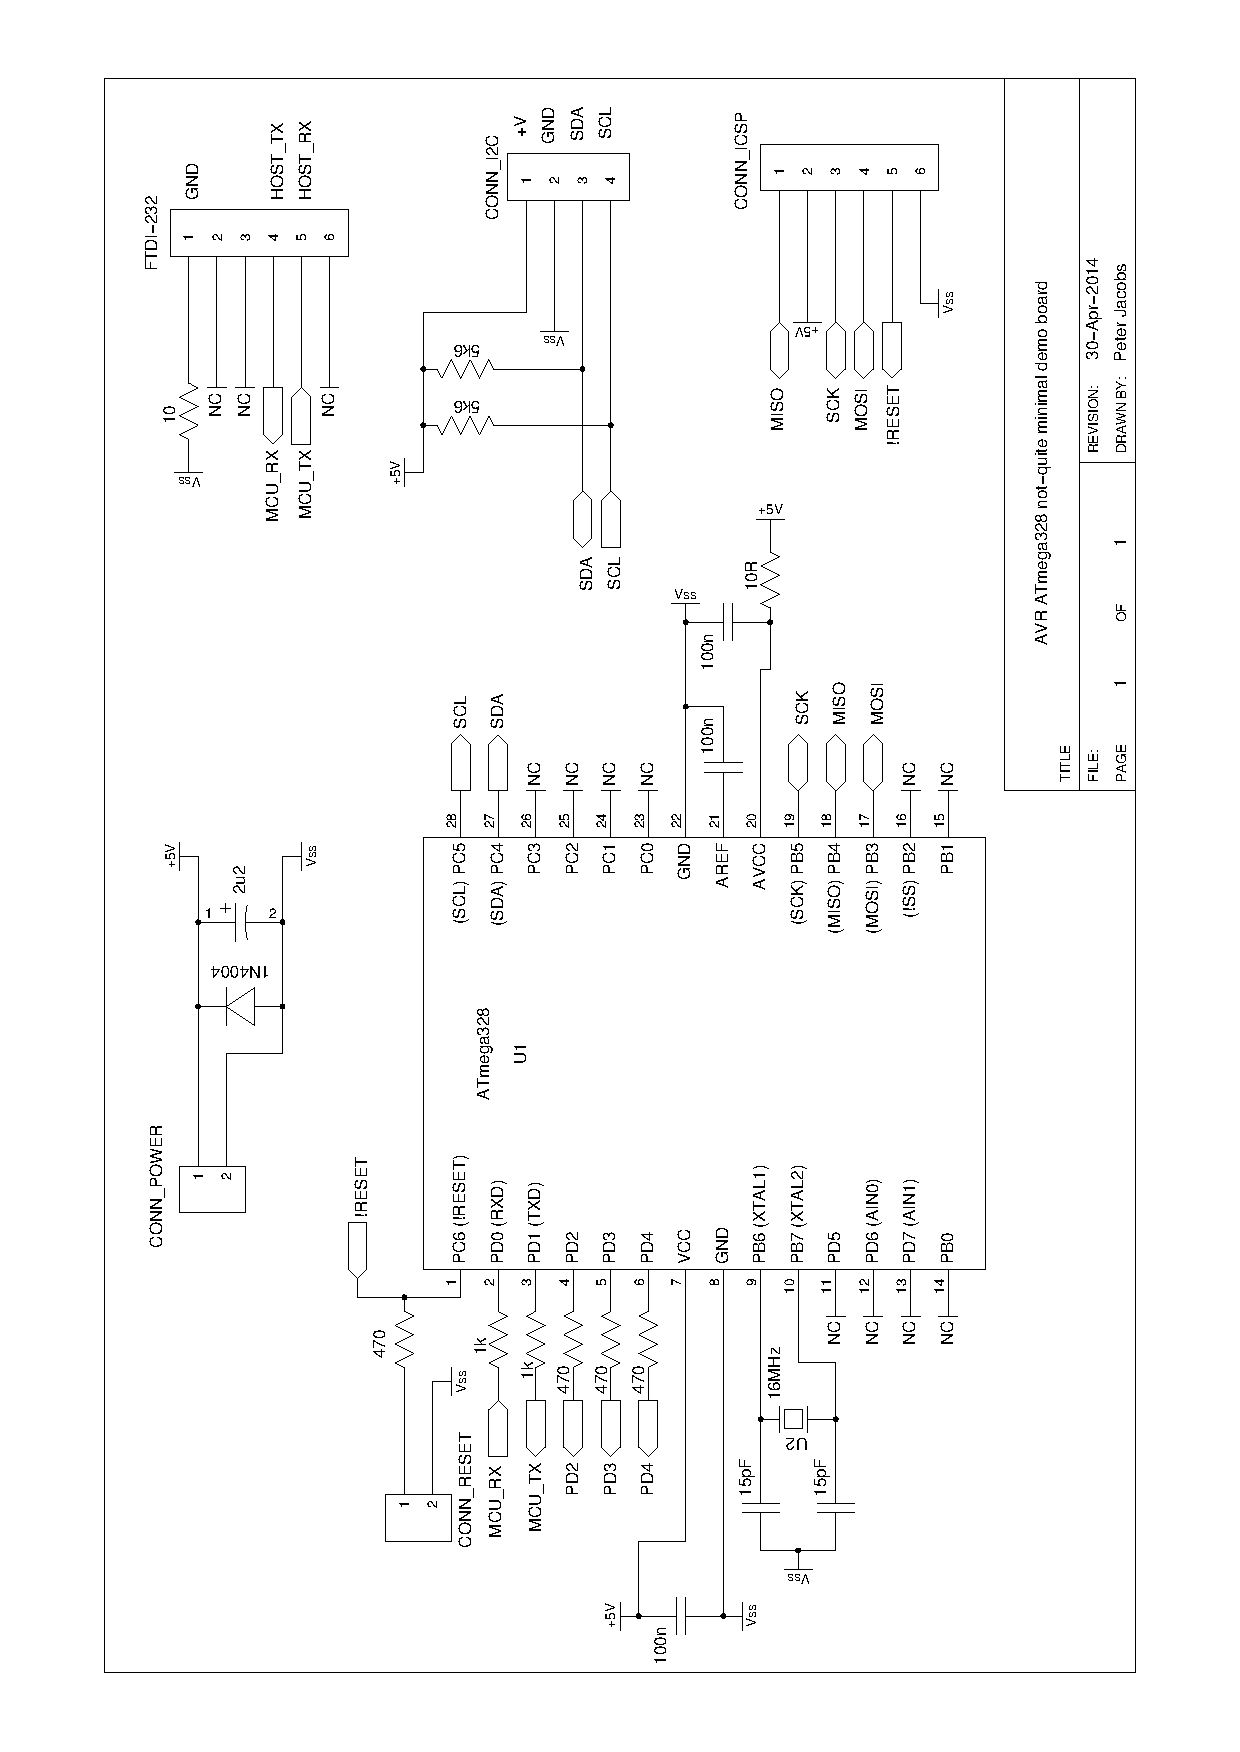
\includegraphics[width=\textwidth,angle=0,viewport=48 37 547 806]{../figs/demo-board-schematic-328.pdf}

\newpage
\noindent
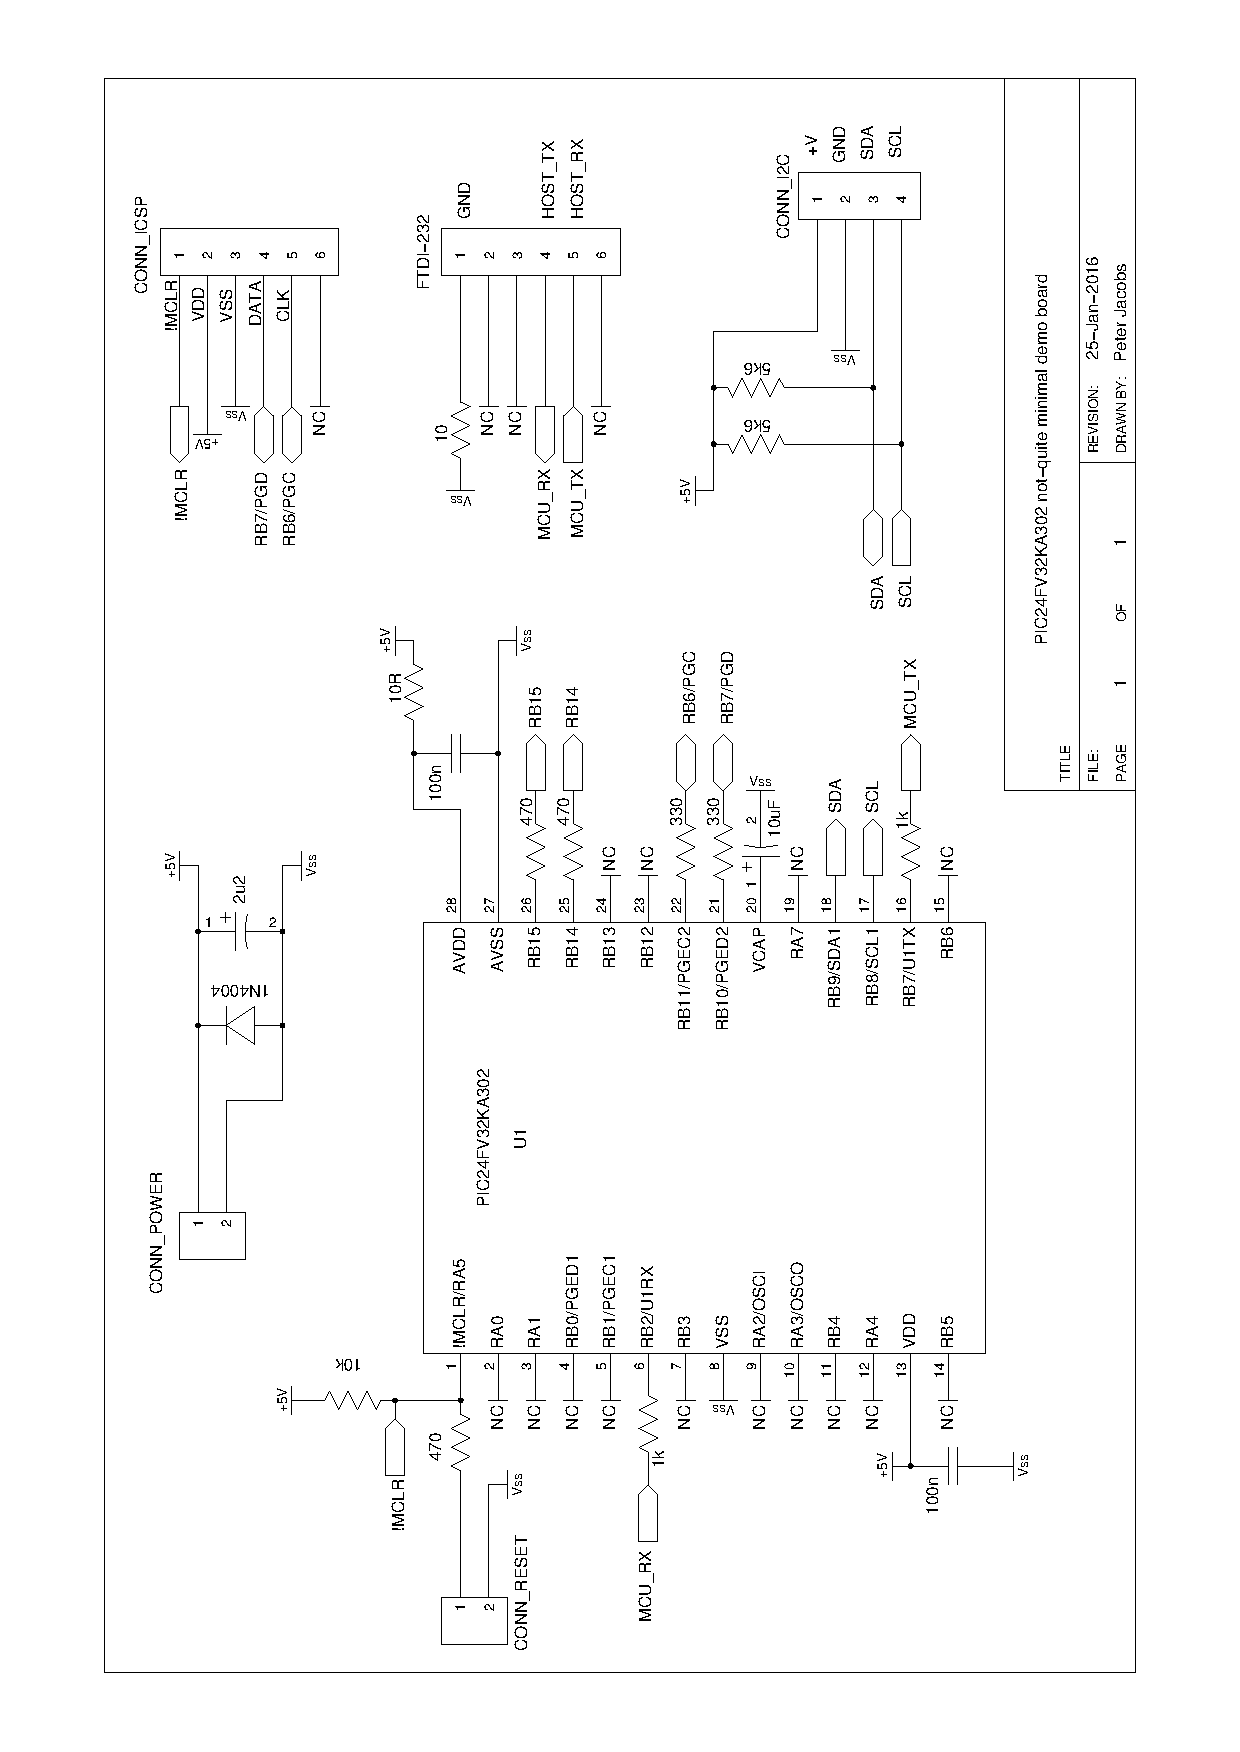
\includegraphics[width=\textwidth,angle=0,viewport=48 37 547 806]{../figs/demo-board-schematic-32ka302.pdf}



\bigskip
\section{FlashForth}
%
Forth is a word-based language, in which the data stack is made available to the programmer
for temporary storage and the passing of parameters to functions.
Everything is either a number or a word.
Numbers are pushed onto the stack and words invoke functions.
The language is simple enough to parse that full, interactive Forth systems may be implemented 
with few (memory) resources.
Forth systems may be implemented in a few kilobytes of program memory and a few hundred bytes
of data memory such that it is feasible to provide the convenience of a fully interactive
program development on very small microcontrollers.

\medskip\noindent
The classic beginners book by Brodie\,\cite{brodie_1987a}
is available online\footnote{\texttt{http://home.iae.nl/users/mhx/sf.html} 
and \texttt{http://www.forth.com/starting-forth/}},
as is Pelc's more recent book\,\cite{pelc_2011a}\footnote{\texttt{http://www.mpeforth.com/}}.
A more detailed reference is published by Forth Inc\,\cite{conklin_rather_2007a}.
These books are biased toward Forth running on a personal computer rather than on
a microcontroller, however, they are a good place to start your reading. 
For an introductory document that is specific to FlashForth, 
see the companion report\,\cite{jacobs_etal_2013b}.

\medskip\noindent
FlashForth\,\cite{nordman_2014a} for the PIC18, PIC24 and ATmega families of microcontrollers 
is a full interpreter and compiler that runs entirely on the microcontroller.
It is a 16-bit Forth with a byte-addressable memory space.
Even though there are distinct memory types (RAM, EEPROM and Flash) and 
separate busses for data and program memory in these Harvard-architecture
microcontrollers, FlashForth unifies them into a single 64kB memory.

\medskip\noindent
Above working in assembler, FlashForth does use some resources, both memory and compute cycles, 
but it provides such a nice, interactive environment that these costs are usually returned 
in convenience while tinkering with your hardware.
Forth programs are very compact so you will have less code to maintain in the long run.
The interpreter can also be available to the end user of your instrument, possibly
for making parameter adjustments or for making the hardware versatile by having a 
collection of application functions present simultaneously in the firmware, 
with the user selecting the required function as they wish.


\bigskip
\subsection{Getting FlashForth and programming the MCU}
%
FlashForth is written in assembler, with one program source for each of 
the microcontroller families and a number of Forth text files to augment the
core interpreter.
The source code can be downloaded from SourceForge at the URL\\
\texttt{http://sourceforge.net/projects/flashforth/}\\
There, you will see that you can get a packaged release or you can clone the git repository.

\medskip\noindent
To build from this source, you will need to start up your integrated development environment 
(be it MPLAB, MPLAB-X or AVR Studio), open the program source and config files in this IDE 
and edit the config file(s) to match your selection of oscillator.
There are other options to customize but the choice of oscillator is the main one.
The machine code can then be assembled and programmed into your microcontroller with 
a suitable device programmer (PICkit3, ICD3, STK500, AVRISP MkII, ...).
Once programmed with FlashForth, and mounted in a board that provides power and serial
communications as described in the previous section, you will be ready to interact with
FlashForth via a serial terminal or shell.


\medskip
\subsection{Building for the PIC18F26K22 or PIC18F46K22}
%
For our minimal system with either the PIC18F26K22 or PIC18F46K22 microcontroller,
we elect to use the internal (16\,MHz) oscillator multiplied by 4 by the PLL.
Within the \verb!MPLAB-X! development environment, 
we started a new standalone project to build our FlashForth program
that will use the microcontroller's UART serial port as the OPERATOR communications channel.
Following the prompt screens, we selected a specific processor (PIC18F26K22), 
our hardware tool (ICD3), and the compiler toolchain (mpasm).

\medskip\noindent
To build the actual machine code that will be programmed into the flash memory
of the microcontroller,
it is sufficient to assemble the principal source file \verb!ff-pic18.asm!
along with the configuration (or header) files \verb!pic18f-main.cfg!, \verb!pic18fxxxx.cfg!, \verb!p18f2x4xk22.cfg!,
and use the linker script \verb!FF_0000.lkr!.
The source file and config files can be found in the directory \verb!pic18/src/!,
while the linker file is in \verb!pic18/lkr/!.
There may be other configuration files already added to the project but you can ignore them.

\medskip\noindent
We edited the processor-specific config file, \verb!p18f2x4xk22.cfg!, writing ``\verb!PLLCFG = ON!'' 
to have the PLL enabled (giving $F_{OSC} = 64$\,MHz),
enable the watchdog timer with a 1:256 postscale (\verb!WDTPS = 256!) 
to get approximately a 1 second time-out period,
and enable the external reset capability (\verb!MCLRE = EXTMCLR!).
Being able to reset the microcontroller by bringing the \verb!MCLR! pin low is something that
we find convenient when tinkering with new hardware.
We set the final line as \\
\verb!#define PLL ENABLE!

\medskip\noindent
We needed to edit the \verb!pic18f-main.cfg! file only to set the system clock frequency
as \verb!constant clock=d'64000000'!.
With this clock frequency, the microcontroller requires approximately 7\,mA current while
the interpreter is running and waiting for input.

\medskip\noindent
There are many other options for customizing the FlashForth program in this file,
however, the default parameters are fine for the first build of our minimal system.
To see your options for all of the configuration bits for your specific microcontroller, 
it is convenient to open the MPLAB-X view from the main menu:
\verb!Window! $\rightarrow$ \verb!PIC Memory Views! $\rightarrow$ \verb!Configuration Bits!.


\medskip\noindent
With the specific microcontroller selected for the project, the config file
\verb!pic18fxxxx.cfg! will automatically select the appropriate MPLAB include file for 
the microcontroller, be it \verb!p18f26k22.inc! for the 28-pin chip on the home-made board
or \verb!p18f46k22.inc! for the 40-pin chip on the PICDEM 2 PLUS board.
If the build process complains of not being able to find the MCU-specific include file,
you may need to adjust the case-sensitivity of the assembler.
This check box can be found in the Project Properties dialog, 
under ``General Options'' for the \verb!mpasmx! assembler, as shown in the following screen shot. 

\bigskip
\noindent
\begin{center}
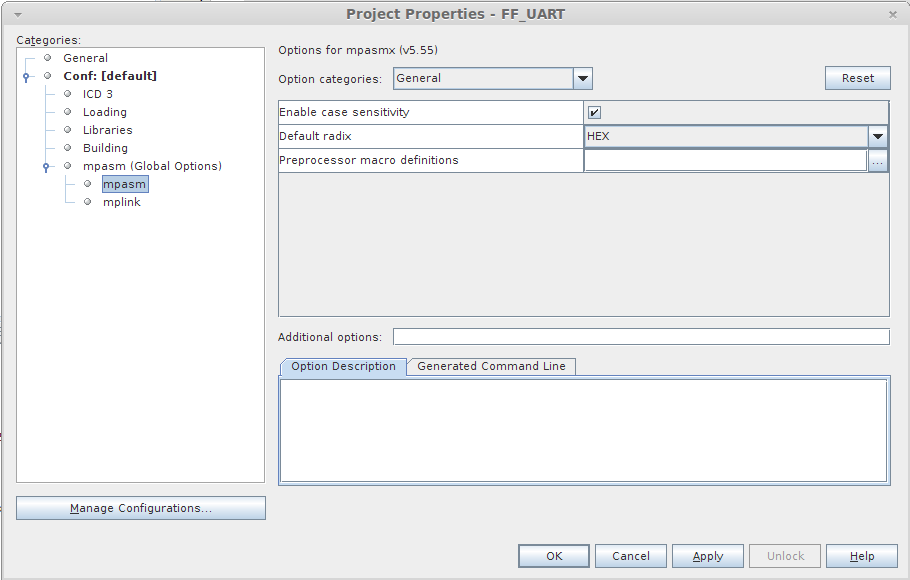
\includegraphics[width=0.6\textwidth]{../figs/MPLAB-X-mpasm-case-sensitivity.png}
\end{center}

\medskip\noindent
The following image shows the result of building in Microchip's MPLAB X IDE.
The lower left frame in the MPLAB-X window shows the MCU resources used.
With 426 bytes of SRAM used (another 3470 free) and 
8948 bytes of program memory used (56588 free),
For the PIC18F26K22 MCU, FlashForth occupies only about one-seventh of 
the microcontroller's program memory.
Most of the memory is available for your application.
For more details on the SRAM memory map, 
see the FlashForth 5 Quick Reference \cite{jacobs_2016b}.
There, Mikael Nordman has provided a memory map that shows how
the SRAM memory is allocated within the FlashForth system. 

\bigskip
\noindent
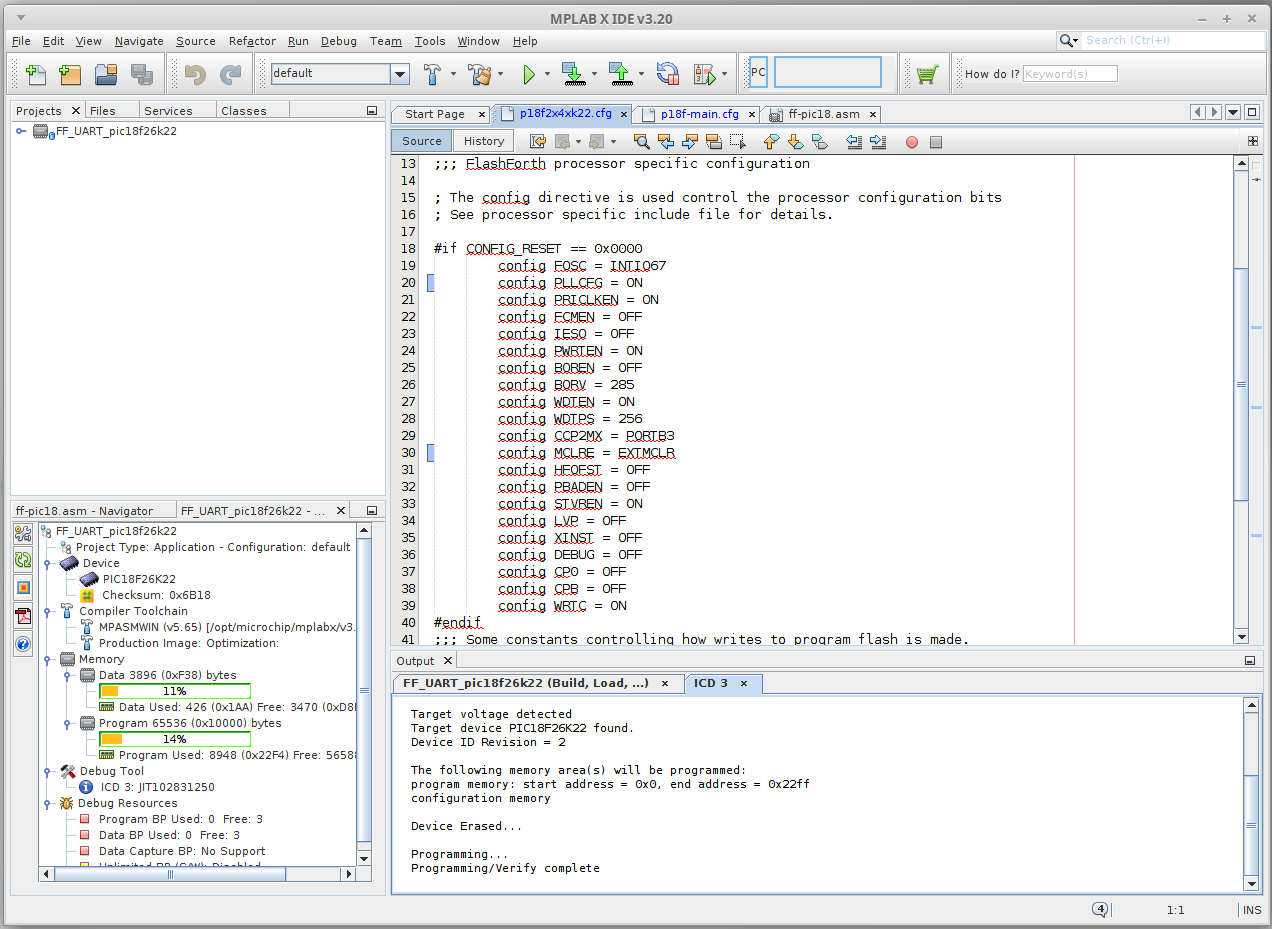
\includegraphics[width=\textwidth]{../figs/MPLAB-X-build-of-Flash-Forth-for-PIC18F26K22-2016.png}

\medskip\noindent
The final step is to program the FlashForth machine code into the flash memory of the microcontroller,
using whatever device programmer you happen to have plugged into your development system.
The Dashboard view in the screen shot above shows that we have seleted to use of the MPLAB ICD3.


\medskip
\subsection{Building for the PIC24FV32KA302}
%
Building for the 16-bit PIC24 family is similar process.
This time look for the source code files in the \verb!pic24/! subdirectory.
There are fewer config files but you may need to customize the closest one for 
your particular processor.  
Here is the required text in the \verb!p24fk_config.inc! file 
for our PIC24FV32KA302-I/SP microcontroller using its internal 8\,MHz oscillator
with 4$\times$ PLL
and installed on the home-made minimal board:

\noindent
{\scriptsize
\begin{verbatim}
;;; Device memory sizes. Set according to your device.
;;; You can increase the addressable flash range be decreasing the addressable ram.
;;; Below is the setting for max amount of ram for PIC24FV32KA302
.equ FLASH_SIZE,     0x5800  ; Flash size in bytes without the high byte
                             ; See program memory size in the device datasheet.
.equ RAM_SIZE,       0x0800  ; Ram size in bytes
.equ EEPROM_SIZE,    0x0200  ; Eeprom size

; For some reason the normal config macros did not work
           .pushsection __FOSCSEL.sec, code
           .global __FOSCSEL
__FOSCSEL: .pword FNOSC_FRCPLL
           .popsection
; Start additions for FF Tutorial board with PIC24FV32KA30x
           .pushsection __FOSC.sec, code
           .global __FOSC
__FOSC:    .pword OSCIOFNC_OFF
           .popsection
           .pushsection __FICD.sec, code
           .global __FICD
__FICD:    .pword ICS_PGx2
           .popsection
; End additions	   

.equ FREQ_OSC, (8000000*4)	 ;Clock (Crystal)frequency (Hz)
\end{verbatim}
} % end scriptsize

\medskip\noindent
Once programmed, FlashForth uses 542 of the microcontroller's 2048 bytes of SRAM and
4544 of the MCU's 11264 words of Flash memory.
This leaves most of the memory for your Forth application program.
Although this appears to be a lot less than that available in the PIC18F26K22 MCU,
this 16-bit MCU has lots of interesting hardware.
With instruction cycle frequency of 16\,MHz and the interpreter waiting for input,
the current consumption is 7.5\,mA, approximately the same as for the 8-bit PIC18F26K22. 


\medskip
\subsection{Building for the ATmega328P}
%
Assembling the FlashForth program within the AVR Studio IDE is fairly simple but
Mike Nordman has made life even simpler for users of Arduino-like hardware by providing
a prebuilt \verb!.hex! file that can be programmed into the ATmega328P.
Here is the command for doing so with avrdude on a Linux PC.
\begin{verbatim}
$ sudo avrdude -p m328p -B 8.0 -c avrisp2 -P usb -e \
  -U efuse:w:0x07:m \
  -U hfuse:w:0xda:m \
  -U lfuse:w:0xff:m \
  -U flash:w:ff_uno.hex:i
\end{verbatim}
The fuses are set to use the 16\,MHz crystal on the Arduino-like board.


\bigskip
\section{Interacting with FlashForth}
\label{interacting-with-flashforth-sec}
%
Principally, interaction with the programmed MCU is via the serial port.
For the PIC microcontrollers, settings are 38400 baud 8-bit, no parity, 1 stop bit, with
software (Xon/Xoff) flow control.
For the ATmega328P (as programmed above), the baud rate is 9600.

\medskip\noindent
The FlashForth distribution includes a couple of shell programs that are 
programmed with some knowledge of the FlashForth interpreter. 
The \verb!ff-shell.py! program is written in Python and allows interaction
with the microcontroller via a standard command shell.
It depends on a Python interpreter and the pyserial extension being installed on your PC.
The \verb!ff-shell.tcl! is a GUI program that displays the interaction text in a dedicated window on your PC.
It requires the Tcl/Tk interpreter which is usually part of a Linux environment but it may be
installed on MS-Windows or MacOSX as well.

\medskip\noindent
The following images shows the \verb!ff-shell.tcl! window just afer sending the content
of the \verb!flash-led.txt! file to the PIC18F26K22.
The device name of \verb!/dev/ttyUSB0! on the status line refers to the USB-to-serial interface 
that was plugged one of the PC's USB ports.
It is convenient to start the program with the command
\begin{verbatim}
$ sudo ./ff-shell.tcl 
\end{verbatim}
If necessary, you can adjust the communication settings by typing new values into the entry boxes 
and pressing \verb!Enter! to repoen the connection.

\bigskip
\noindent
\begin{center}
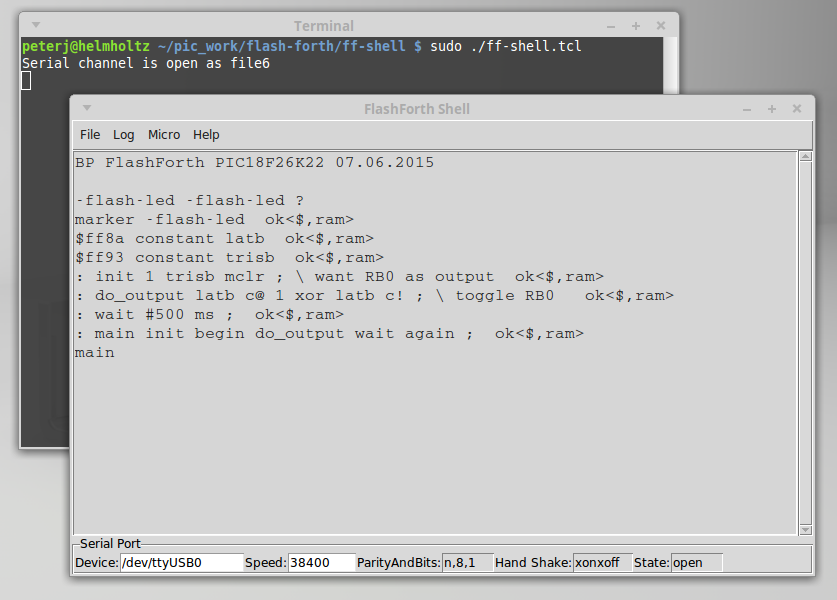
\includegraphics[width=0.7\textwidth]{../figs/ff-shell-tcl-flash-led-pic18.png}
\end{center}

\medskip\noindent
As you type characters into the main text widget, \verb!ff-shell.tcl! intercepts them and sends them, 
one at a time, via the serial port to the microcontroller.
As the microcontroller sends characters back, the program filters them and displays them in the text widget.
There is also a send-file capability that will send the text from the file
as fast as it can, without overwhelming the microcontroller.
The Python program \verb!ff-shell.py! has a special command \verb!#send! to start the equivalent process.

\medskip\noindent
If you have sent the microcontroller off to do a repetitive task, such as flashing the LED indefinitely,
you can regain the interpreter's attention by sending a \verb!Control-O! character.
The interpreter aborts the execution of the current word and does a software restart. 
After initialization, the interpreter announces that it is ready to begin.
Subsequently pressing \verb!Enter! will get the \verb!ok! response, as shown below.
The warm restart action is also available from the menu as \verb!Micro!$\rightarrow$\verb!Warm Restart!.

\bigskip
\noindent
\begin{center}
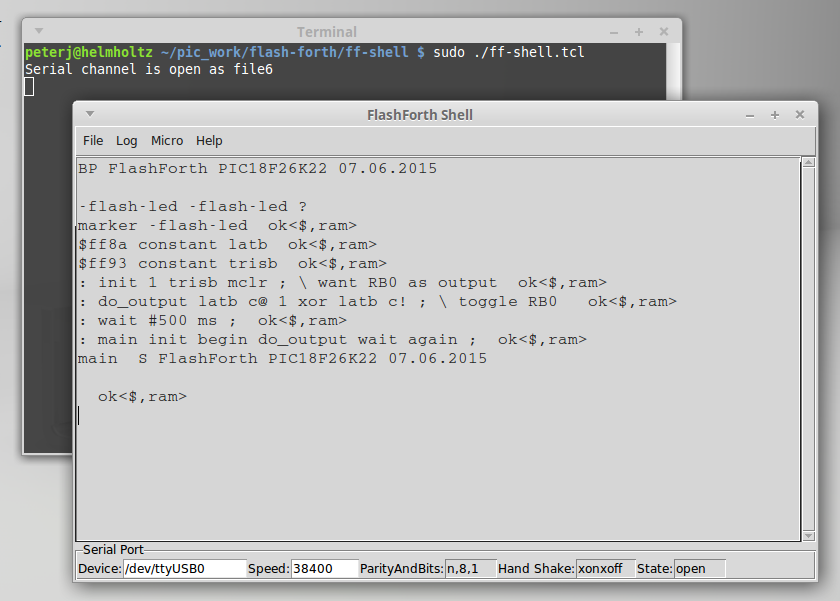
\includegraphics[width=0.7\textwidth]{../figs/ff-shell-tcl-control-O-pic18.png}
\end{center}

\medskip\noindent
We find \verb!ff-shell.tcl! a very convenient interaction environment, however,
if you want to use a standard terminal program on Linux or MacOSX, 
Appendix \ref{other-terminal-programs-sec} provides a few notes for doing so.


\newpage
\section{Introductory examples}
%
We begin with examples that demonstrate a small number of features of the MCU 
or of FlashForth.
Our interest will primarily be in driving the various peripherals of the MCU
rather than doing arithmetic or dealing with abstract data.

\subsection{Hello, World: Flash a light-emitting diode with the PIC18}
%
The microcontroller version of the ``Hello, World'' program is typically a program that
flashes a single LED.
It will work on either of PIC18F microcontrollers mentioned previously and 
makes use of a digital input-output pin via the registers that control the IO port.
The datasheet\,\cite{pic18f26k22-datasheet} has a very readable introduction 
to the IO ports.
Please read it.

\bigskip\noindent
\code{}{../pic18/flash-led-pic18.txt}

\medskip\noindent
Notes on this program:
\begin{itemize}
 \item If the word \verb!-flash-led! has been previously defined with the word marker, 
  line 1 resets the dictionary state and continues interpreting the file, 
  else the interpreter signals that it can't find the word and continues interpreting the file anyway.
 \item Line 2 records the state of the dictionary and defines the word \verb!-flash-led!
  so that we can reset the dictionary to its state before the code was compiled, 
  simply by executing the word \verb!-flash-led!.
 \item Lines 3 and 4 define convenient names for the addresses of 
  the special function registers (SFRs) that control IO-port B.
  Note the literal hexadecimal notation with the \verb!$! character.
  In the PIC18F family, the SFRs appear near the top of the 64k FlashForth memory space.
 \item Line 5 is a colon definition for the word \verb!init! that sets up the peripheral
  hardware.  
  Here, we set pin RB0 as output.
  The actual command that does the setting is \verb!mclr!,
  which takes a bit-mask (00000001) and a register address (\verb!$ff93!)
  and then clears the register's bits that have been set in the mask.
  Note the comment starting with the backslash character. 
  Although the comment text is sent to the MCU, it is ignored.
  Note, also, the spaces delimiting words.  That spaces after the colon and
  around the semicolon are important.
 \item Line 6 is the definition that does the work of fiddling the LED pin.
  We fetch the byte from the port B latch, toggle bit 0 and 
  store the resulting byte back into the port B latch.
 \item Line 7 defines a word to pause for 500 milliseconds.
  Note the \verb!#! character for a literal decimal integer.
 \item Line 8 defines the ``top-level'' coordination word, which we have named
  \verb!main!, following the C-programming convention.
  After initializing the relevant hardware, it unconditionally loops, doing the output
  operation and waiting, each pass.
 \item Line 9 invokes the \verb!main! word and runs the application.
  Pressing the \verb!Reset! button will trigger a hardware restart,
  kill the application and put the MCU back into a state of listening to the serial port.
  Invoking a warm restart by typing \verb!Control-O! or selecting the \verb!Warm Restart! 
  menu action in \verb!ff-shell.tcl! may be a more convenient way to stop the application.
  Typing \verb!main!, followed by \verb!Enter! will restart the application.
\end{itemize}

\medskip\noindent
Instead of going to the bother of tinkering with the MCU IO Port, 
we could have taken a short-cut and used the string writing capability 
of Forth to write a short version that was closer the the operation of
typical Hello World programs.

\medskip\noindent
\code{}{../src/short-hello-world.txt}

\medskip\noindent
Before going on to more examples, it is good to know about the word \verb!empty!.
This word will reset the dictionary and all of the allotted-memory pointers.
Because FlashForth does not allow you to redefine words that are already in the dictionary,
later examples that use the same names for their word definitions, 
may not compile without complaint if you don't clean up after each exercise.


\bigskip
\subsection{Flash a light-emitting diode with the PIC24}
%

\noindent
\code{}{../pic24/flash-led.txt}

\medskip\noindent
Notes on this program:
\begin{itemize}
\item This program for the 16-bit microcontroller is essentially the same as that
  for the 8-bit MCU, with different addresses for the port-control registers, of course.
  In the PIC24/dsPIC30/dsPIC33 version of FlashForth, the special function registers appear
  in the lowest 2k bytes of memory.
\item On line 5, we compute the bit pattern for selecting the MCU pin rather than writing it explicitly.
  We start with a 1 in the least-significant bit of the 16-bit word and then shift it left 15 places,
  to produce the binary value \verb!%1000000000000000!
\item On line 7, we use 16-bit fetch \verb!@! and store \verb?!? operations because the
  special function registers for controlling the hardware on this microcontroller are 16 bits wide.
\end{itemize}


\bigskip
\subsection{Flash a light-emitting diode with the ATmega}
%

\noindent
\code{}{../avr8/flash-led-avr.txt}

\medskip\noindent
Notes on this program:
\begin{itemize}
\item Again, except for the specific registers and bits, 
  this program is the same as for the other MCUs.
  As for other high-level languages, we no longer have to think
  about the specific machine architecture (usually).
\item Because we are using load and store instructions, 
  the special function registers start at address \verb!$20!.
\end{itemize}


\newpage
\subsection{Set the cycle duration with a variable (PIC18)}
%
We enhance the initial demonstration by making the waiting period setable.
Because of the interactive FlashForth environment, 
the extra programming effort required is tiny.
The appearance of the code, however, looks a bit different because we have 
laid out the colon definitions in a different style and have included 
more comments.

\bigskip\noindent
\code{}{../pic18/flash-led-var.txt}

\noindent
Notes on this program:
\begin{itemize}
 \item If the file has been sent earlier defining the application's words,
  line 1 resets the state of the dictionary to forget those previous definitions. 
  This makes it fairly convenient to have the source code open in an editing window
  (say, using \verb!emacs!) and to simply reprogram the MCU by resending the file
  (with the \verb!Send-File! menu item in \verb!ff-shell.tcl!). 
 \item Line 7 defines a 16-bit variable \verb!ms_count!.
 \item Line 30 leaves the wait period on the stack before invoking the \verb!main! word.
 \item On each pass through the \verb!wait! word, the 16-bit value is fetched from
  \verb!ms_count! and is used to determine the duration of the pause.
\end{itemize}


\newpage
\subsection{Hello, World: Morse code}
%
Staying with the minimal hardware of just a single LED attached to pin \verb!RB0! 
on the PIC18F26K22 or PIC18F46K22, 
we can make a proper ``Hello World'' application.
The following program makes use of Forth's colon definitions so that we can 
spell the message directly in source code and 
have the MCU communicate that message in Morse code.

\bigskip\noindent
\code{}{../pic18/hello-world.txt}

% \noindent
% Notes on this program:
% \begin{itemize}
%   \item
% \end{itemize}


\newpage
\section{Read and report an analog voltage}

\subsection{PIC18FX6K22}
%
Use of the analog-to-digital converter (ADC) is a matter of, first,
reading Section 17 of the PIC18F2X/4XK22 datasheet\,\cite{pic18f26k22-datasheet},
setting the relevant configuration/control registers and then giving it a poke
when we want a measurement.
Again, the interactive nature of FlashForth makes the reporting 
of the measured data almost trivial.

\bigskip\noindent
\code{}{../pic18/read-adc.txt}

\noindent
Notes on this program:
\begin{itemize}
 \item Although not much needs to be done to set up the ADC, 
  you really should read the ADC section of the datasheet
  to get the full details of this configuration.
 \item Lines 17 to 19 uses binary literals (with the \verb!%! character) 
  to show the configuration bits explicitly.
 \item Line 24 conditionally repeats testing of the DONE bit for the ADC.
 \item Line 25 fetches the full 10-bit result and leaves it on the stack
  for use after the \verb!adc@! word has finished.  
  Because of the selected configuration of the ADC peripheral, 
  the value will be right-justified in the 16-bit cell.
 \item Line 35 invokes the \verb!adc@! word and prints the numeric result.
 \item Line 37 checks if a character has come in from the serial terminal.
  If so, the loop is terminated and the main function returns control to
  the FlashForth interpreter.
\end{itemize}

\bigskip

\subsection{PIC24FV32KA30X}
%
The analog-to-digital converter on the PIC24-series microcontrollers is a little more complex
than that on the PIC18 series.
There are more features to select and so there are more registers and bits to set, however, 
the essential set-up tasks are similar.
The following script sets up some word definitions that were developed with a view to using them 
in a larger program. 
The particular words are more verbose but also carry more information.

\bigskip\noindent
\code{}{../pic24/read-adc-pic24.txt}

\noindent
Notes on this program:
\begin{itemize}
  \item This script was part of a larger application for the monitoring of 2 pressure transducers, 
    hence the setting up of just RA0 and RA1 at the start of \verb!adc.init! at lines 38--41.
  \item To save power the peripheral modules of a PIC24 are, by default, disabled.
    You need to clear a module's disable bit (line 42) to do anything with it, 
    even setting configuration registers.
    The (separate) power-on bit still needs to be set to start up the converter.
\end{itemize}

\bigskip

\subsection{ATmega328P}
%
Although the analog-to-digital converter on the ATmega328P is different in detail,
it has essentially the same functionality that can be abstracted.
To control the ADC module, we can set up the same words 
(\verb!adc.init!, \verb!adc.close!, \verb!adc.select! and \verb!adc@!) 
as for the PIC24FV32KA302.

\bigskip\noindent
\code{}{../avr8-2016/read-adc-avr.txt}

\noindent
Notes on this program:
\begin{itemize}
  \item Although there are 6 analog pins available, the test word only exercises channels 0 and 1.
  \item The input channel selection is controlled by the lower bits in the \verb!admux! register.
    Other than the 6 external analog input pins, you can select:
    \begin{itemize}
     \item the temperature sensor with bit pattern \verb!%1000!,
     \item the internal band-gap reference with \verb!%1110!, and
     \item and the zero-volt rail (GND) with \verb!%1111!.
    \end{itemize}
\end{itemize}


\newpage
\section{Counting button presses}
%
Example of sensing a button press, with debounce in software.

\bigskip\noindent
\code{}{../pic18/push-button.txt}

\noindent
Notes on this program:
\begin{itemize}
  \item The \verb!main! word clears the \verb!count! variable, calls \verb!init! to set up the hardware
   and then loops, polling \verb!RB0! and incrementing value of the \verb!count! variable only when 
   the button gets pressed.
  \item If the pause after acknowledging the button press (line 42) is too long,
    we may lose later button press events.  
    This depends on how frantically we press S3.
  \item Line 44 resets the watch-dog timer on each pass of the main loop.
    If we don't press the RB0 button for a long time, the main loop would not otherwise pause 
    and clear the watch-dog timer.
    The watch-dog timer is cleared inside the \verb!ms! word, however,
    if the timer expires before being cleared, the microcontroller would be reset
    and the FlashForth interpreter would restart.    
\end{itemize}


\newpage
\section{Counting button presses via interrupts}
%
Instead of polling the \verb!RB0! pin attached to the push button, as in the previous example,
let's set up the hardware interrupt mechanism to invoke the increment action for us.

\bigskip\noindent
\code{}{../pic18/pb-interrupt.txt}

\noindent
Notes on this program:
\begin{itemize}
  \item Again, we use the variable named \verb!count! as the variable to be incremented
   on pressing the button that pulls RB0 low.
   The actual increment is done on line 19, inside the interrupt service word \verb!int0-irq!.
   The second variable, \verb!last-count!, is used on line 36 in the \verb!main! word,
   to detect when the \verb!count! variable changes.
  \item The \verb!init! word sets up the bits to enable the \verb!INT0! external interrupt
   to fire on a falling edge at RB0.
  \item On line 28 in the \verb!init! word, the execution token for our interrupt service word
   is stored as the high-priority interrupt vector.
   Because FlashForth supports only high-priority interrupts, the \verb!0! is a dummy value 
   but is still expected by the \verb?int!? word.
  \item Inside the interrupt-service word, we need to test the \verb!INT0IF! interrupt flag
   to see if it is our interrupt to handle and, if it is, do the appropriate work 
   (of incrementing the \verb!count! variable) and clearing the interrupt flag.
   If you enable several interrupt sources, you need to provide a test and action for each.
  \item The \verb!main! word clears the \verb!count! variable, calls \verb!init! to set up the interrupt
   mechanism and then loops, emitting the value of the \verb!count! variable only when it changes.
\end{itemize}


\newpage
\section{Scanning a 4x3 matrix keypad}
\label{4x3-keypad-section}
%
We connect a 4x3 matrix keypad to PORTB, using RB0, RB1 and RB2 to drive the columns 
while sensing the rows with RB4 through RB7.
The schematic figure below shows the arrangement of keys and pins.

\medskip
\centerline{
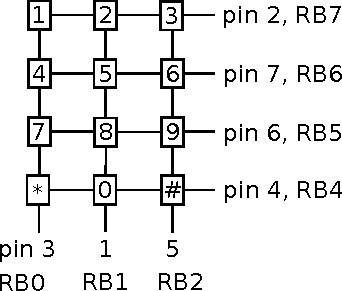
\includegraphics[height=4cm]{../figs/keypad-4x3-portb.pdf}
}

\medskip\noindent
To minimize hardware, we have used the weak pull-ups on PORTB.
Pressing a key while its column wire is held high does nothing, however,
pressing a key on a column that is held low will result in its row
being pulled low.

\bigskip\noindent
\code{}{../pic18/keypad.txt}

\noindent
Notes on this program:
\begin{itemize}
  \item In lines 21--31, we make use of character arrays to store (into the program memory)
    the the ASCII code and the scan code for each key.
    The scan code is made up of the 3-bit column pattern to be applied to RB2-RB0 and the
    resulting 4-bit row-sense pattern (RB7-RB4) expected for the particular key if it is pressed.
    RB3 is maintained high (and is of no consequence) for this 3-column keypad, however, 
    it would be used for a 4x4 keypad.
  \item Lines 36 and 47 make use of the for--next control construct to work through 
    the set of 12 scan codes.
  \item We should go further by making use a state-machine 
    and also keeping track of the last key pressed.
\end{itemize}


\newpage
\section{Communicating with SPI devices}
%
The photograph below shows the Eleven AVR board driving a matrix display.
This particular display board has an 8$\times$8 LED matrix being controlled by
a MAX7219 8-digit LED display driver \cite{max7219-datasheet}.

\medskip
\centerline{
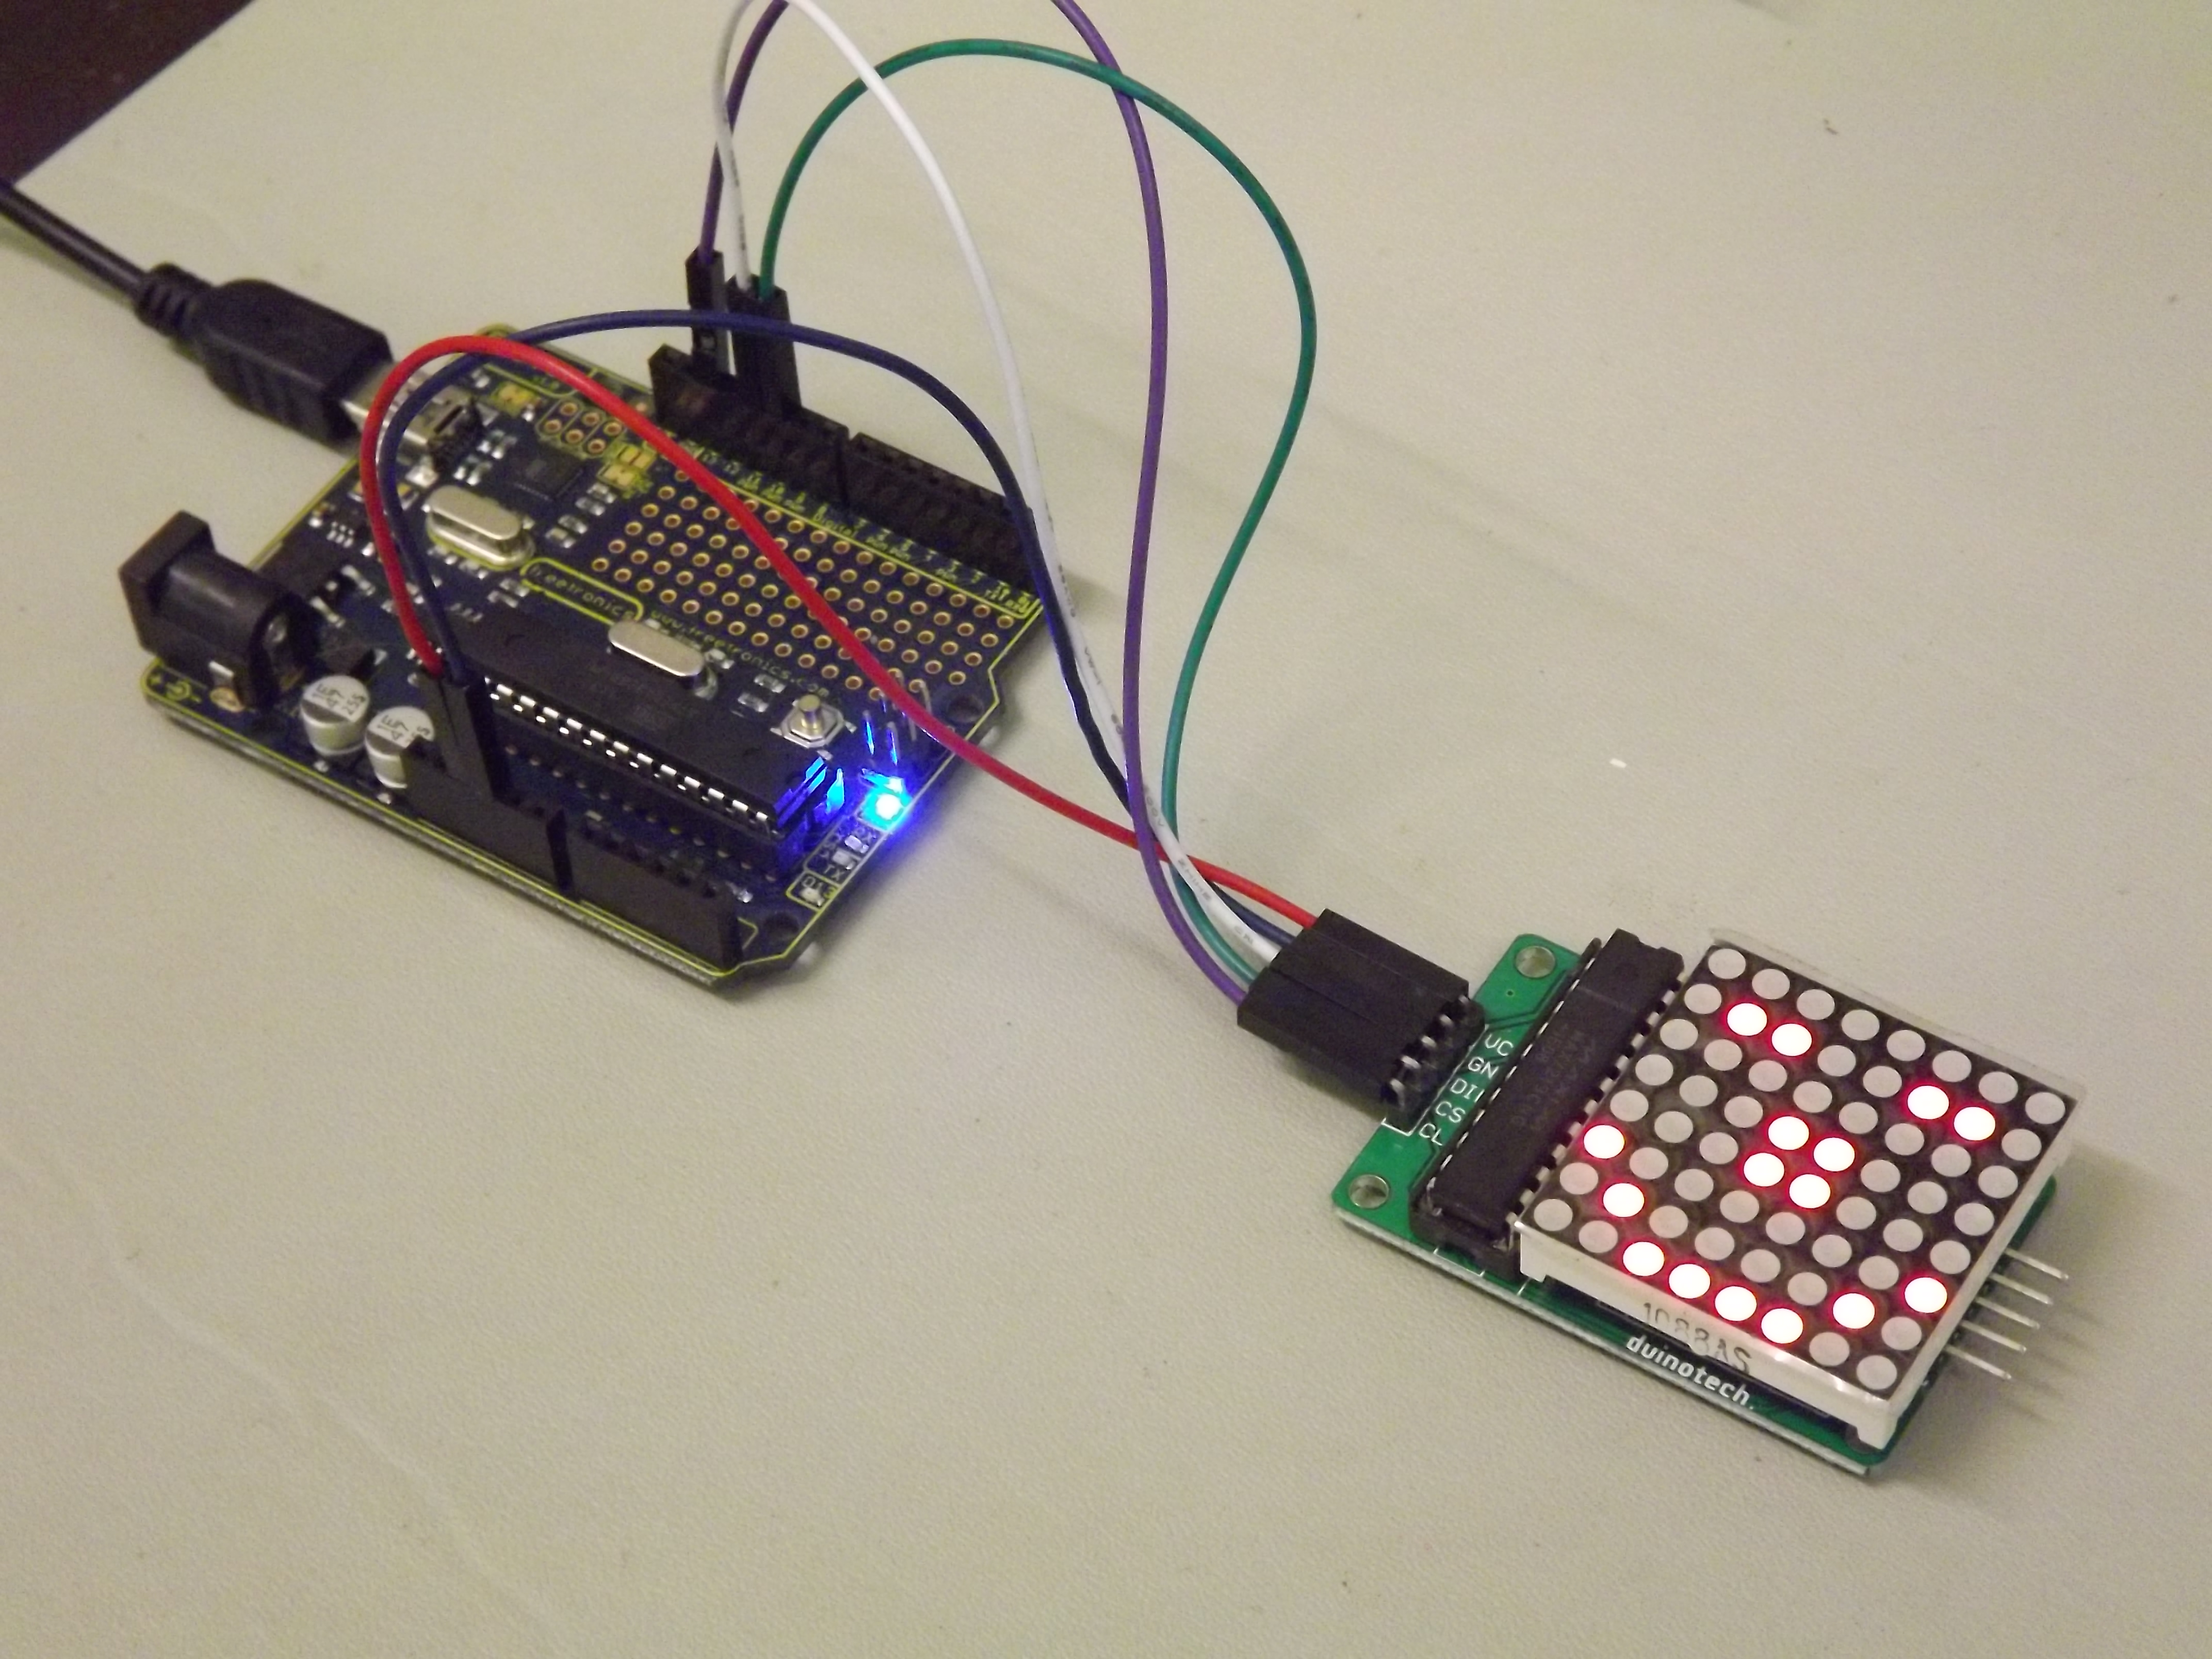
\includegraphics[height=5cm]{../figs/eleven-driving-MAX7219-LED-matrix.jpeg}
}

\medskip\noindent
The MAX7219 has a serial data interface that can be driven by the SPI module
within each of the microcontrollers.
The timing diagram, taken directly from the datasheet \cite{max7219-datasheet}, 
is shown below, along with the expect format for each 16-bit command.
A command can be sent to the MAX7219 chip by taking the chip-select line low,
sending two bytes via the SPI module and then taking the chip-select line high.
A set of words for doing this 2-byte transfer and building the higher-level commands
on top of that transfer is given in Section\,\ref{driving-max7219-sec}.

\medskip
\centerline{
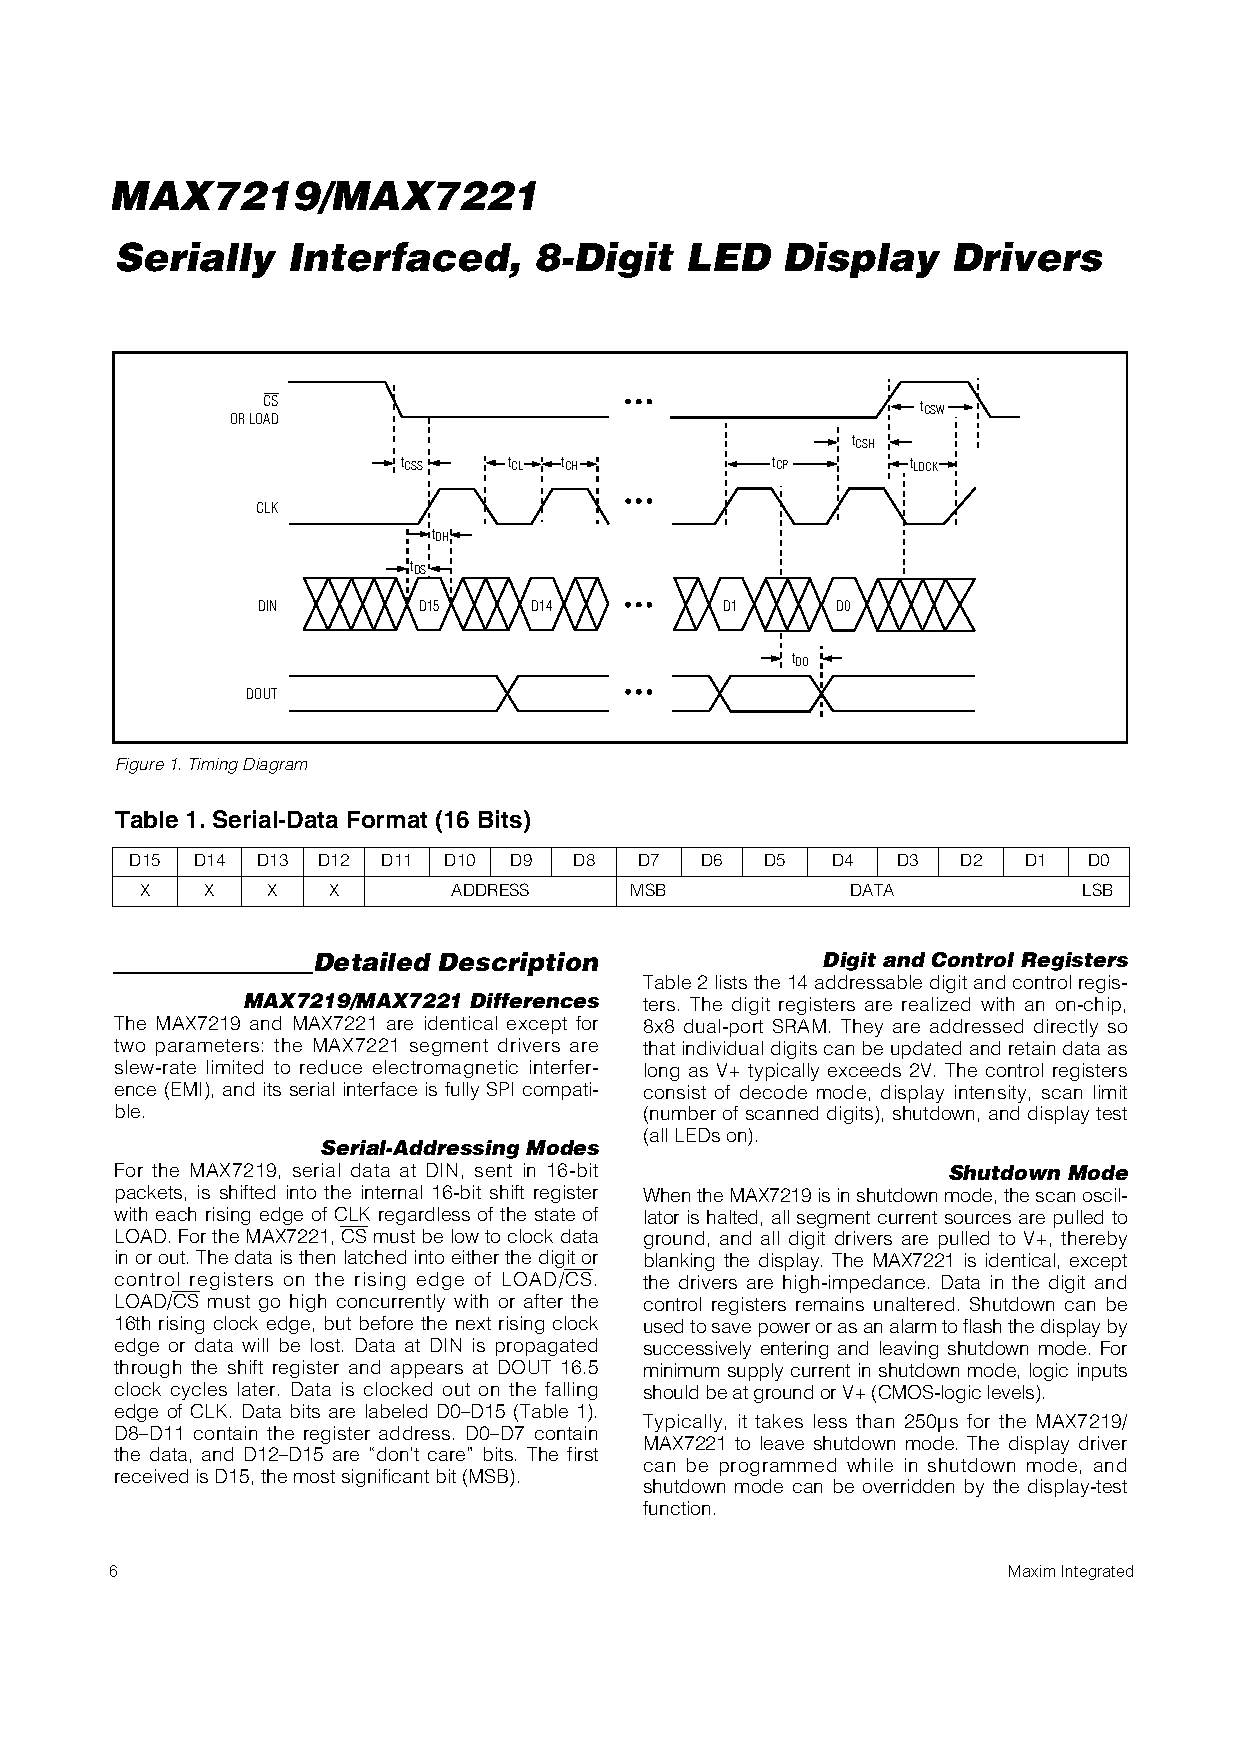
\includegraphics[width=\textwidth,viewport=53 407 543 675,clip=true]{../figs/max7219-timing-diagram.pdf}
}

\medskip\noindent
The following sections define the words for using SPI peripherals for each of the microcontrollers 
in master mode.
The SPI module is initialized for mode 0 operation, with clock signal idling low, 
and data lines changing as the clock signal transitions from active to idle. 
This suits the MAX7219, which samples the data as the clock signal transitions from idle to active. 
These words provide abstract the hardware registers and bits to provide a common vocabulary for the interaction
with SPI slave devices.

\subsection{PIC18FX6K22}
%

\medskip\noindent
\code{}{../pic18/spi2-base-k22.txt}

\noindent
Notes on this program:
\begin{itemize}
  \item For the PIC18F26K22, we choose to use the second SPI module 
    because we have the pins associated with the first module assigned to the I$^2$C communications,
    as discussed in Section\,\ref{i2c-sec}.
  \item Lines 40 and 41 activate the weak pull-up for the MISO pin.
    Some slave devices, such as the MAX7219, do not have a data-out pin to talk back to the master.
  \item The key word \verb!spi.cexch! starts the exchange of a byte by writing it to the SPI data buffer.
    On completion of the transfer, detected by the interrupt flag going high,
    the incoming byte is fetched from the same buffer.
    If there is no data line connected to the MISO pin, a byte of all 1s will be returned.
    If you know that is the expected, it may be convenient to use the \verb!spi.csend! which
    does the same exchange but then drops the incoming byte.
\end{itemize}

\subsection{PIC24FV32KA30X}
\code{}{../pic24/spi1-base-pic24fv32ka302.txt}

\noindent
Notes on this program:
\begin{itemize}
  \item On this microcontroller, we choose to use the first SPI module, again because
    it results in a convenient set of pins.
    Section\,\ref{i2c-sec} uses the I$^2$C pins on \verb!RB5! and \verb!RB6!.
  \item On lines 43 through 46, the SPI1 module is configured to behave much like the 
    8-bit SPI module on the PIC18F26K22.
    If we didn't care about making a common set of words for the three example processors
    in this tutorial guide, 
    we would probably make use of the advanced features on this 16-bit microcontroller.
    These features include 16-bit transfer and enhanced buffering.
\end{itemize}

\subsection{ATmega328P}
\code{}{../avr8-2016/spi-base-avr.txt}

\noindent
Here is a screenshot showing the record of the SPI communication pins on the ATmega328P 
as it sends the single byte \verb!$0c$!, as specified in the \verb!spi-test! word.
The SPI clock period is 1 microsecond.

\medskip
\centerline{
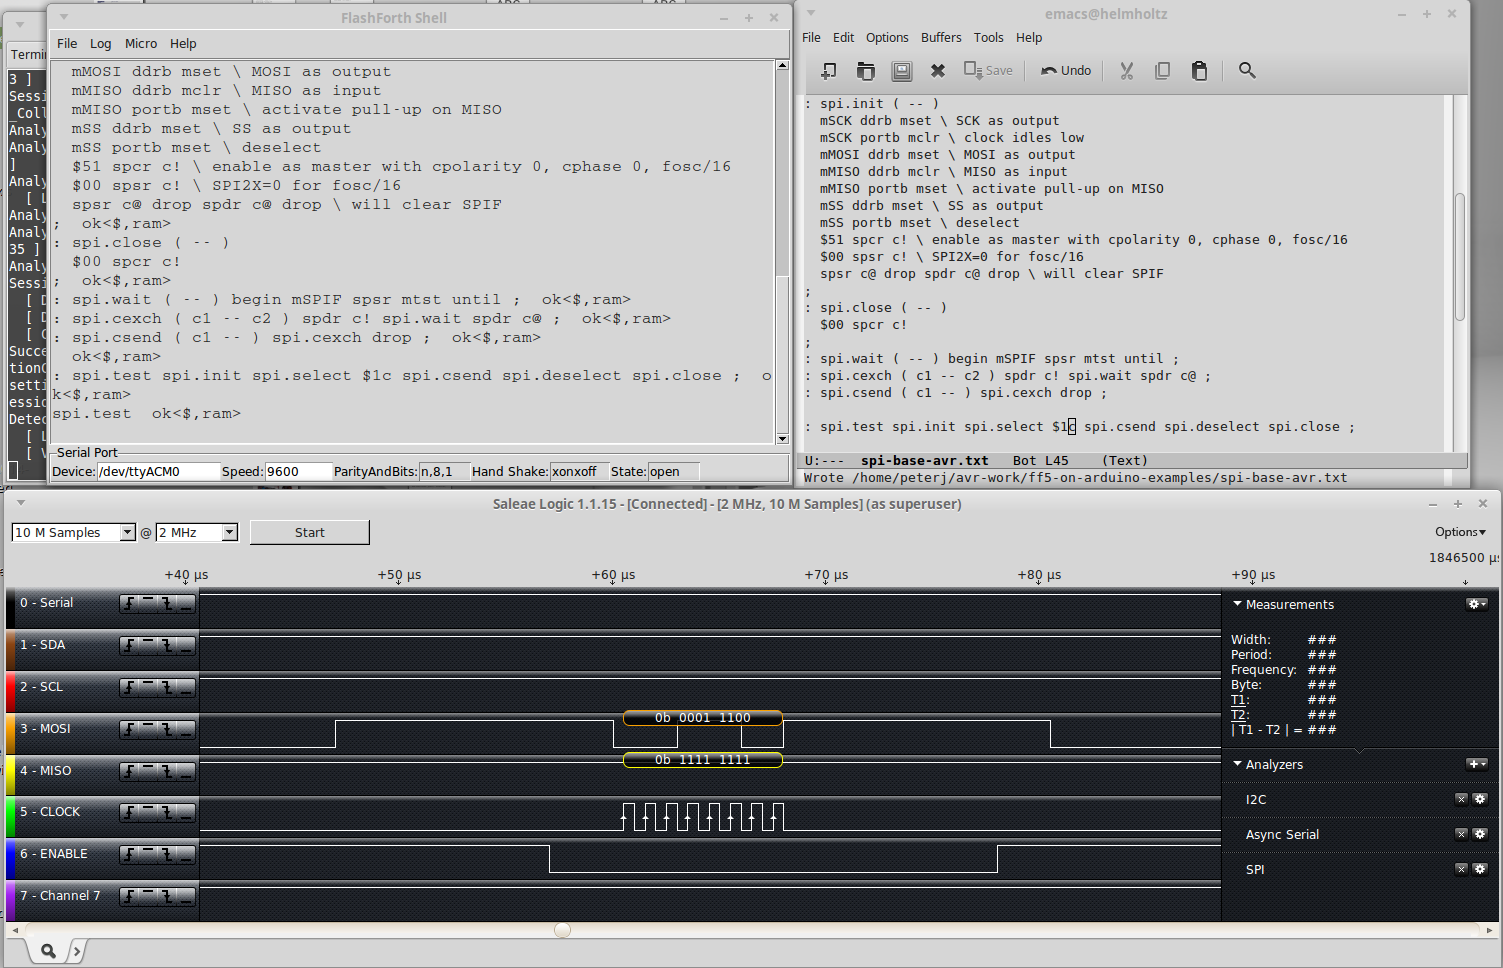
\includegraphics[width=\textwidth]{../figs/eleven-spi-test-avr-sending-0c-byte.png}
}

\newpage

\subsection{Words to drive a matrix display}
\label{driving-max7219-sec}
%
Given the base words defined in the previous sections, any of the boards may drive the
matrix display with the following words.
The interesting commands are defined by line 20 and 
the \verb!disp-test-X! words are three examples of doing something with the display.

\medskip\noindent
\code{}{../avr8-2016/led-matrix-display.txt}


\newpage
\section{Communicating with I2C devices}
\label{i2c-sec}
%
Here are some words for using I$^2$C (or Two-wire) peripherals for each of the microcontrollers in master mode.
These words provide abstract the hardware registers and bits to provide a common vocabulary for the interaction
with I$^2$C slave devices.

\subsection{PIC18FX6K22}
\code{}{../pic18/i2c-base-k22.txt}

\subsection{PIC24FV32KA30X}
\code{}{../pic24/i2c-base-pic24fv32ka30x.txt}

\subsection{ATmega328P}
\code{}{../avr8-2016/i2c-base-avr.txt}

\subsection{Notes on using the words}
\begin{itemize}
  \item The word \verb!i2c.init! is used to set up the I$^2$C master peripheral for further activities.
  \item I$^2$C conversations begin by addressing a slave device for either reading or writing.
    The words \verb!i2c.addr.read! and \verb!i2c.addr.write! are provided for this waking of the slave.
    They leave a flag on the stack to indicate whether the slave device acknowledged being addressed.
    If the slave device responded appropriately, you may proceed to read or write bytes.
  \item There are two words for reading a byte from the bus.  
    \verb!i2c.c@.ack! reads a byte and asserts an acknowledge (ACK) to indicate to the slave device that
    another byte will be read subsequently.
    \verb!i2c.c@.nack! reads a byte and asserts a NACK to indicate to the slave that no more bytes are wanted.
  \item The word to send a byte to the slave device is \verb?i2c.c!?.
    This word leaves a flag to indicate the state of the ACK bit following the action of sending the byte.
    If the slave asserted ACK, the flag will be \verb!0!.
    You may \verb!drop! this flag if it not of interest to you.
  \item There are lower-level words \verb!i2c.start!, \verb!i2c.rsen! and \verb!i2c.stop! to assert
    start, restart and stop conditions respectively.
    These are used within the higher-level words mentioned above.
  \item The utility word \verb!i2c.ping?! attempts to address a slave and read a byte.
    It leaves \verb!true! if the slave responds, else \verb!false!.
  \item Sometimes when tinkering with a new I$^2$C device,
    you can get into a state of confusion such that the slave device will end up in some intermediate state
    waiting for clock signals.\footnote{This happens more often than I would like to admit.}
    In this state, the slave device will no longer respond in a way that the master peripheral understands.
    Rather than cycle the power to reset the slave device, it may be convenient to force the clocking
    of the data bits through the bus and get the slave device back into an idle state.
    The word \verb!i2c.reset.bus! (in i2c-base-pic24fv32ka30x.txt) is provided to automate this
    forced clocking.
\end{itemize}

\newpage

\subsection{Detecting I2C devices}
%
Building on the base words for a particular microcontroller, the following program works on
all of the microcontrollers discussed in this tutorial guide.
It is convenient to run this program to to see if the device of interest is responding.
There's no point trying to have a conversation with a device that doesn't respond to being addressed.  

\bigskip\noindent
\code{}{../pic18/i2c-detect.txt}

\newpage

\section{Using I2C to get temperature measurements}
%
Using the words in \verb!i2c-base-k22.txt! to control the MSSP peripheral in master mode, 
one may talk to the TC74A5 temperature measurement chip on the PICDEM 2 PLUS
and report sensor temperature.

\bigskip\noindent
\code{}{../pic18/read-tc74-2016.txt}

\medskip\noindent
With a Saleae Logic Analyser connected to the pins of the TC74A5, we can see the I$^2$C 
signals as a result of calling the \verb!tc74-init! word.\\
\rule{0cm}{0.2cm}\\
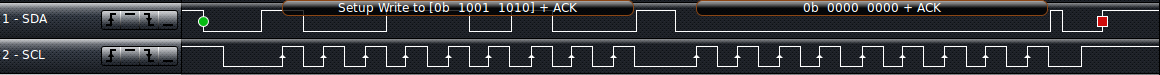
\includegraphics[width=\textwidth]{../figs/saleae-logic-read-tc74-init-binary-region.png}

\medskip\noindent
A little later on, the \verb!degrees@! word is invoked.  
The returned binary value of \verb!0b00010101! corresponds 
to the very pleasant 21$^o$C that exists in the back shed as this text is being written.\\
\rule{0cm}{0.2cm}\\
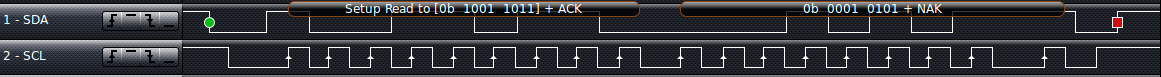
\includegraphics[width=\textwidth]{../figs/saleae-logic-read-tc74-read-binary-region.png}


\newpage
\section{Making high-resolution voltage measurements}
%
The Microchip MCP3422 is a $\Sigma \Delta$-ADC that can connected via I$^2$C port.
This neat little converter can measure voltages with a resolution of 18 bits 
(at the lowest data rate of 3.75 samples per second) and includes
a programmable gain amplifier\,\cite{mcp3422-datasheet}.
Being available in a surface-mount package only, it was convenient to use a prebuilt
evaluation board, the green board between the home-built FlashForth demo board 
and the fixed-voltage supply board.
The MCP3422 evaluation board is connected to and powered from the I$^2$C header on the
FlashForth demo board.  
Separately, the fixed-voltage supply board provides the measurement voltage 
to channel 1 of the MCP3422 via a potentiometer that is set to give 1.024\,V, 
according to my (fairly cheap) multimeter.

\medskip
\centerline{
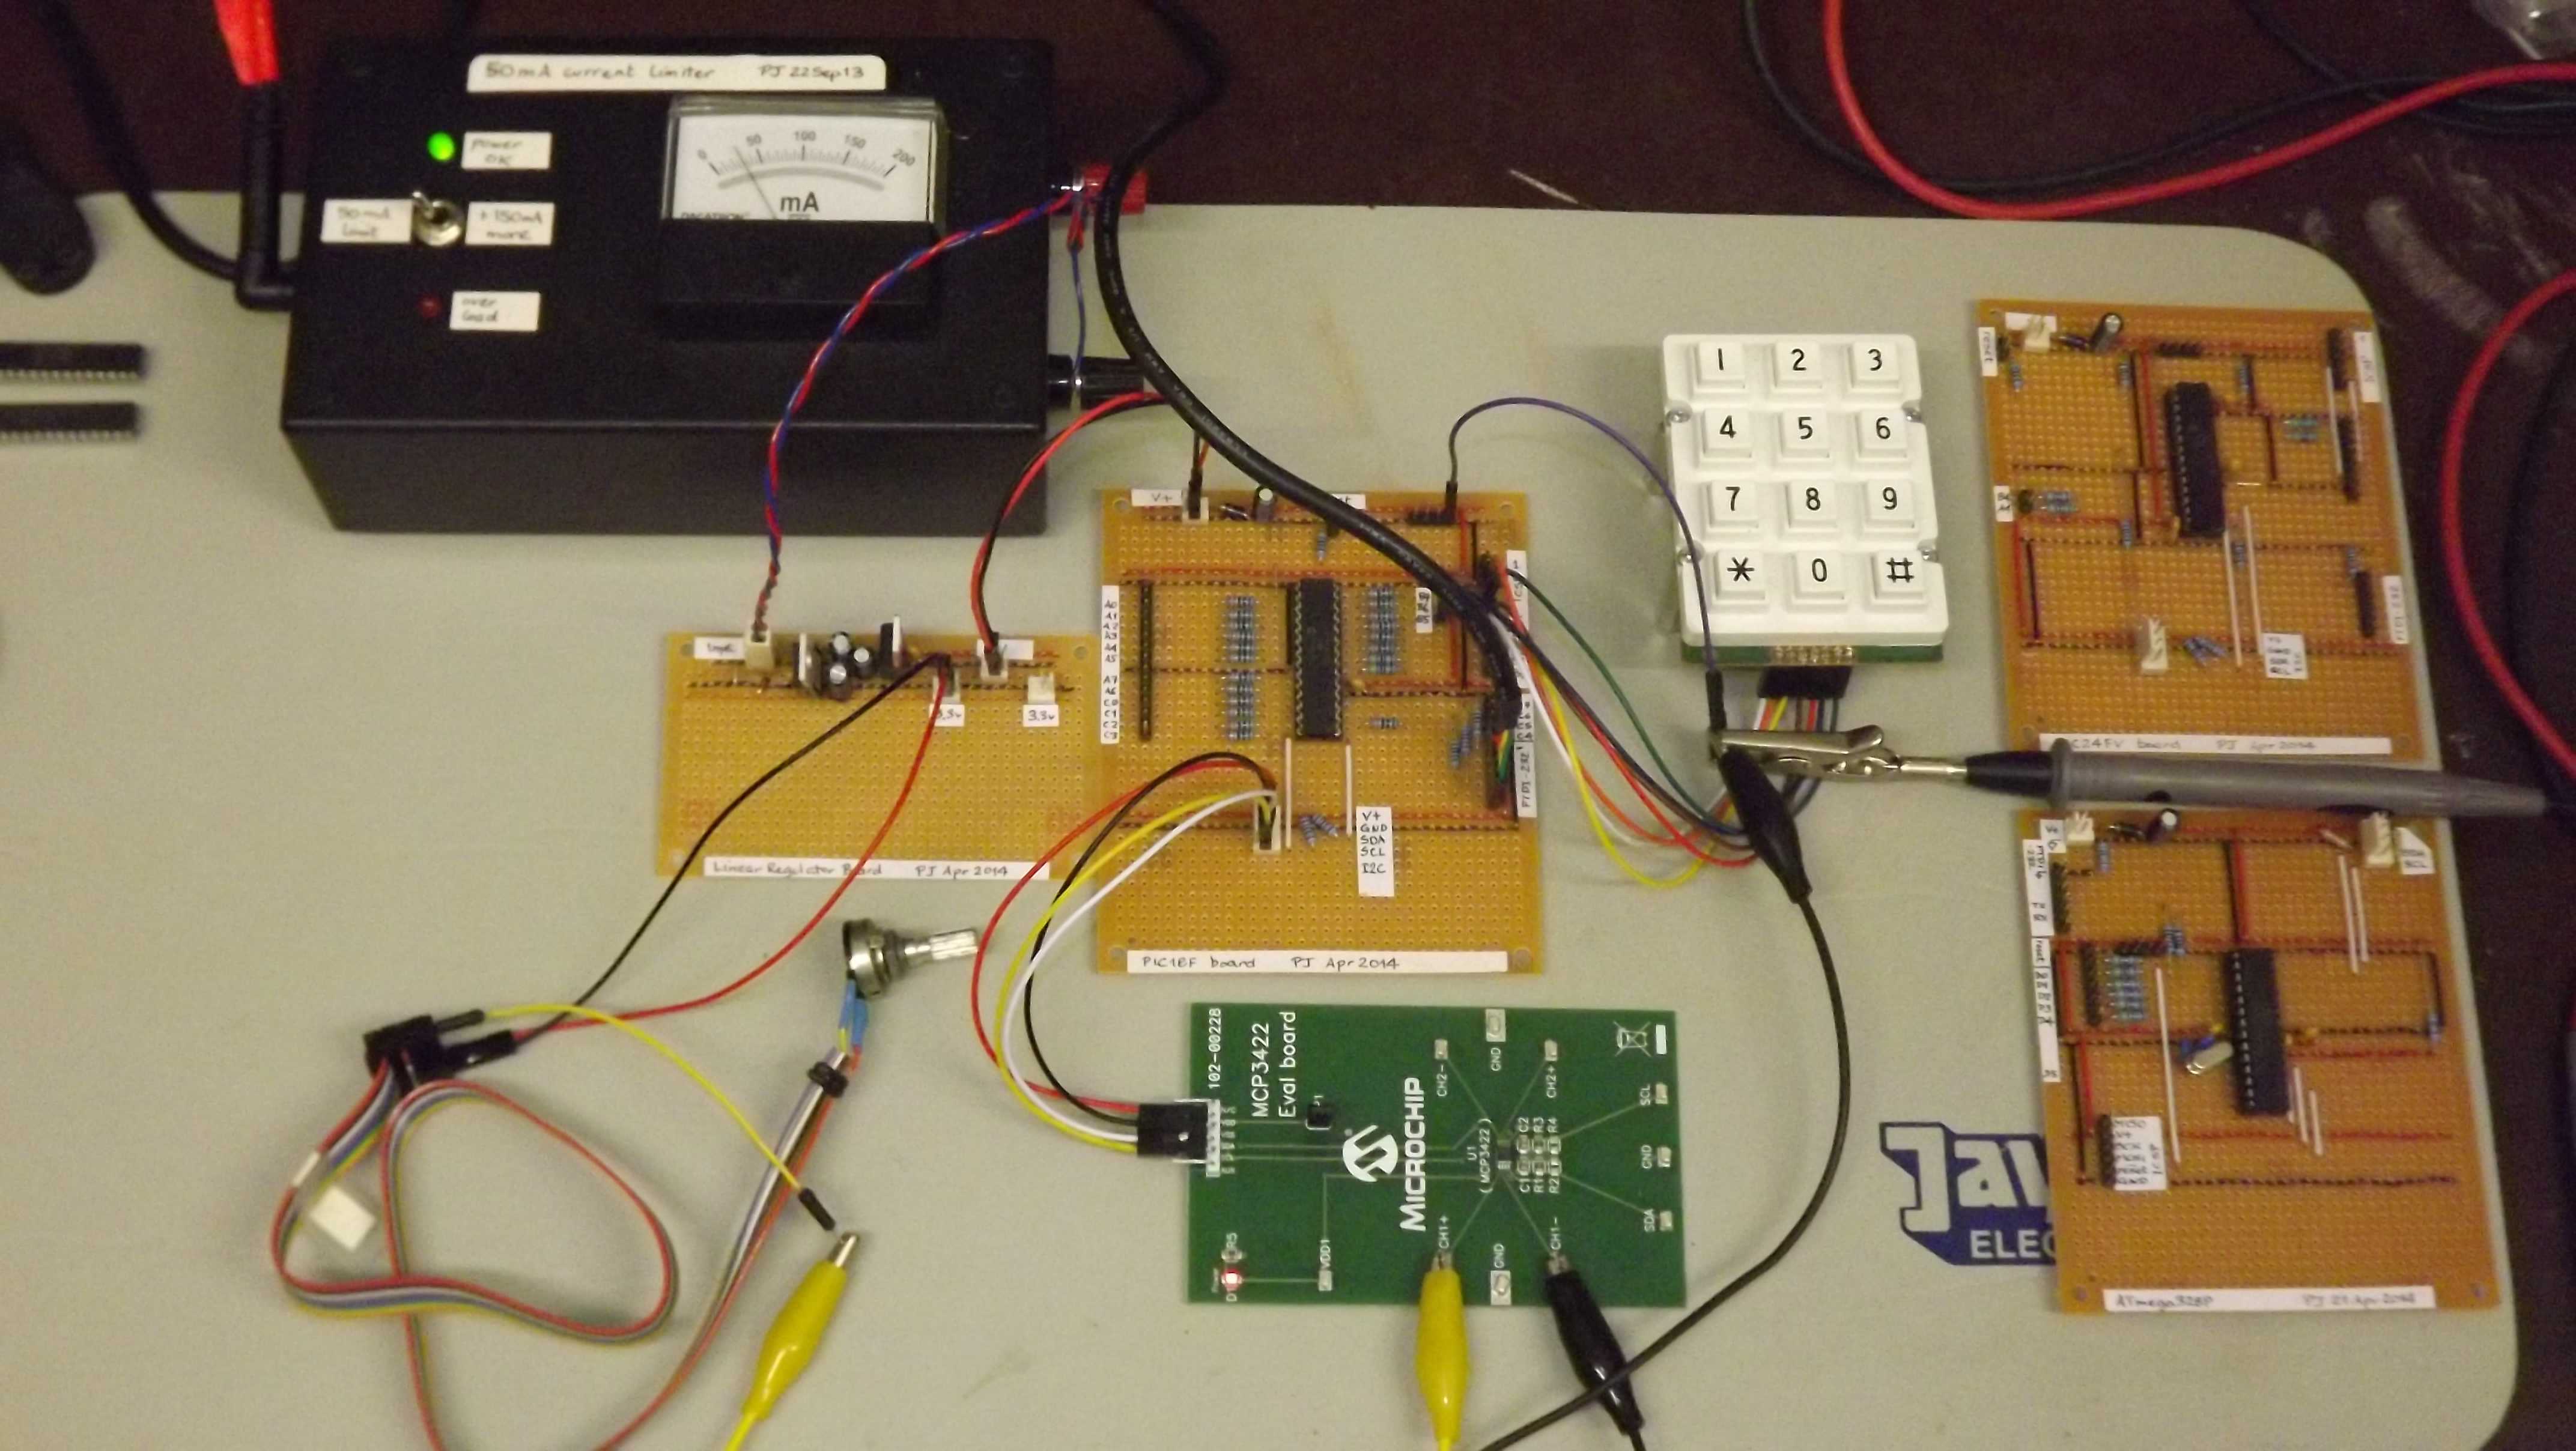
\includegraphics[width=0.9\textwidth]{../figs/mcp3422-i2c-demo-with-pic18f26k22.jpeg}
}

\bigskip\noindent
\code{}{../pic18/mcp3422-2016.txt}

\medskip\noindent

\medskip
\noindent
Notes on this program:
\begin{itemize}
  \item \verb!mcp3422-run! is the top-level word that initializes the hardware, then periodically
    reads the MCP3422 data and reports the voltage (in millivolts) to the user terminal.
    The program runs until a key is pressed.
  \item The converted value is read from the MCP3422 as an 18-bit value in 2-complement format.
    The word \verb!mcp3422@! reads the data as three bytes from the I$^2$C port and then 
    shuffles it into a double-cell value that is left on the stack, along with a flag to indicate
    whether the value sent by the MCP3422 happened to be the latest data.
    If the MCP3422 did not respond to being addressed, zeros will be left on the stack in place
    of the expected data.
  \item The value is scaled to microvolts and then the resultant double value is output using the
    pictured numeric output to have 3 decimal places so that it looks like a millivolt reading.
    Several lines from the terminal look like the following:
    \begin{verbatim}
new 1028.031 mV 
new 1028.062 mV 
new 1028.046 mV 
    \end{verbatim}
  \item This program builds upon the \verb!i2c-base-k22! words
    in order to communicate with the MCP3422. 
    The code for scaling of the measured data requires 
    the mixed-scale word \verb!m*/! from the file \verb!math.txt! provided by FlashForth.
\end{itemize}


% \bigskip
\newpage
\section{An I2C slave example}
%
The MSSP in the PIC18F26K22 can also be used in slave mode.
Here, the FlashForth demo board is presented as an I$^2$C slave device to
an Aardvark serial interface, acting as master.
The UART communication is provided by a Future Technology Devices International
USB TTL-serial cable.

% \medskip
% \centerline{
% \includegraphics[width=0.7\textwidth]{../figs/demo-board-i2c-with-aardvark.jpeg}
% }

\medskip\noindent
The core of the program is the \texttt{i2c\_service} word which is invoked
each time a serial-port event is flagged by the SSPIF bit in the PIR1 flag register.
This word is an implementation of the state look-up approach detailed in 
the Microchip Application Note AN734\,\cite{bowling_raj_2008a}.
The rest of the program is there to provide (somewhat) interesting data 
for the I$^2$C master to read and to do something (light a LED)
when the master writes suitable data to the slave.

%\newpage
\bigskip
\noindent
\code{}{../pic18/i2c-slave.txt}

\medskip\noindent
With a Saleae Logic Analyser connected, we can see the I$^2$C 
signals as a result of writing the byte \texttt{0x01} to turn on the LED.
The following figure shows the data and clock signals from the time that the
master asserts the START condition (green circle) 
until it asserts the STOP condition (as indicated by the red square).\\
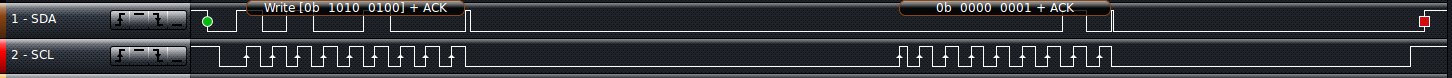
\includegraphics[width=\textwidth]{../figs/i2c-aardvark-write-byte.png} \\
The clock frequency is 100kHz and there is a 138\,$\mu$s gap 
between the ninth clock pulse of the address byte and
the start of the pulses for the data byte.
This gives an indication of the time needed to service each SSPIF event.

\medskip\noindent
A little later on, the Aardvark reads two bytes from the bus, as shown here.\\
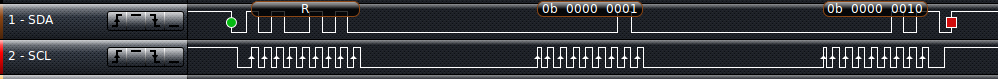
\includegraphics[width=\textwidth]{../figs/i2c-aardvark-read-2-bytes.png}\\
Zooming in, to show the finer annotation, the same signals are shown below.\\
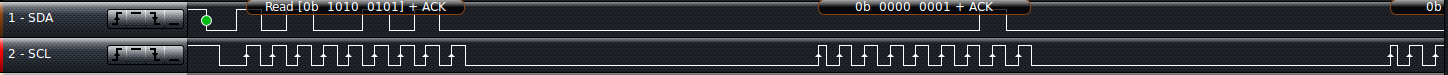
\includegraphics[width=\textwidth]{../figs/i2c-aardvark-read-2-bytes-zoom-to-start.png}\\
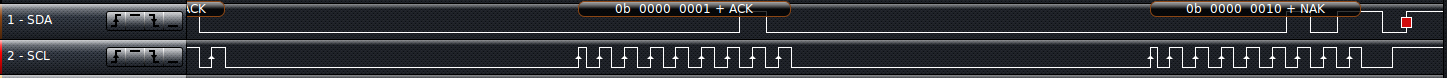
\includegraphics[width=\textwidth]{../figs/i2c-aardvark-read-2-bytes-zoom-to-nack.png}\\
Again, the inter-byte gap is 138\,$\mu$s resulting in about 200\,$\mu$s 
needed to transfer each byte.
This effective speed of 5\,kbytes/s should be usable for many applications,
since the I$^2$C bus is typically used for low speed data transfer.

\medskip
\noindent
Notes on this program:
\begin{itemize}
  \item Need to load \texttt{core.txt} before the source code of the \texttt{i2c-slave.txt}.
  \item Slave examples found in documentation on the Web usually have the service function
    written in the context of an interrupt service routine.
    The MSSP can be serviced quite nicely without resorting to the use of interrupts,
    however, you still have to check and clear the SSPIF bit for each event.
  \item The implementation of the test for State 5 (Master NACK) is slightly
    different to that described in AN734 because it was found that the master
    would assert an I$^2$C bus stop after the final NACK of a read operation
    but before the MCU could service the SSPIF event.
    This would mean that STOP was the most recent bus condition seen
    by the MSSP and the START and STOP bits set to reflect this.
    In the figures shown above, there is only about 12\,$\mu$s between the ninth
    clock pulse for the second read data byte and the Aardvark master asserting 
    the STOP condition on the bus.
    This period is very much shorter than the (approx.) 140\,$\mu$s period 
    needed by the slave firmware to service the associated SSPIF event.
\end{itemize}


%\bigskip
\newpage
\section{Speed of operation -- bit banging}
%
All of this nice interaction and convenience has some costs.
One cost is the number of MCU instruction cycles needed to process
the Forth words.
To visualize this cost, the following program defines a word \verb!blink-forth! which
toggles an IO pin using the high-level FlashForth words that fetch and store bit patterns into the
port latch register.
An alternative word \verb!blink-asm! uses assembler instructions to achieve an equivalent effect, but faster,
and a third word \verb!blink-bits! uses the FlashForth \verb!bit0:! and \verb!bit1:! words
to create high-level bit-manipulation words that also achieve full machine speed.

\subsection{PIC18F26K22}
%

\bigskip\noindent
\code{}{../pic18/speed-test.txt}

\noindent
Notes on this program:
\begin{itemize}
 \item We have had to worry about clearing the watch-dog timer.
  In the early examples, the FlashForth interpreter was 
  passing through the pause state often enough to keep the watch-dog happy.
  The words in this example give the FlashForth interpreter no time to pause
  so we are responsible for clearing the watch-dog timer explicitly.
 \item In the source code config file for the specific MCU, the watch-dog timer postscale
  is set to 256.
  With a 31.25\,kHz oscillator frequency, this leads to a default timeout period
  of a little over 1 second ($32\,\mu{\rm s} \times 128 \times 256$).
 \item For the PIC18 MCU, the internal oscillator of 16\,MHz was multiplied by the PLL
   to get 64\,MHz oscillator driving the MCU.  
   With 4 clock cycles per instruction cycle, this gave an instruction period $T_{CY}=62.5$\,ns.
   Current consumption by the microcontroller was about 14\,mA, roughly double the value
   when the interpreter is not doing much, just waiting for input.
 \item The screen image on the left shows the output signal for running the high-level
  \verb!blink-forth! word while the image on the right uses the assembler words.
  \begin{center}
  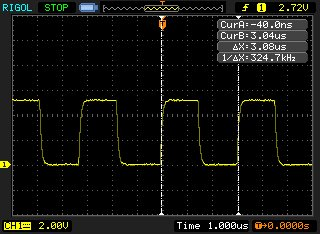
\includegraphics[width=0.45\textwidth]{../figs/speed-test-forth-pic18f26k22.jpeg}
  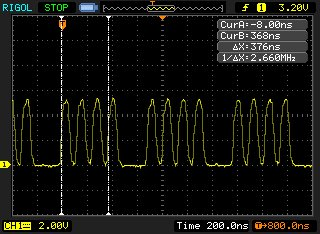
\includegraphics[width=0.45\textwidth]{../figs/speed-test-asm-pic18f26k22.jpeg}
  \end{center}
 \item For the \verb!blink-forth! word, one on+off cycle of the LED executes in 6 words
  and is seen (in the oscilloscope record) to require about 50 instruction cycles.
  So, on average, each of these threaded Forth words is executed in about 8 MCU instruction cycles. 
  Note that this overhead includes the cost of using 16-bit cells for the data.
  Extra machine instructions are used to handle the upper bytes.
  In other applications, where we actually want to handle 16-bit data, 
  this will no longer be a penalty.
 \item The assembler version has no overhead and the cycle time for the MCU
  instructions defines the period of the output signal.
  One on-off cycle requires 2 instructions so we see a short 125\,ns period.
  This is fast enough that the capacitive loading on the output pin 
  is noticeable in the oscilloscope trace.
  Also, the time required for the machine instructions to clear the watch-dog timer
  and the instruction jump back to the start of the loop 
  now shows up clearly in the oscilloscope record.
 \item The oscilloscope record for the \verb!blink-bits! word is shown here.
  \begin{center}
  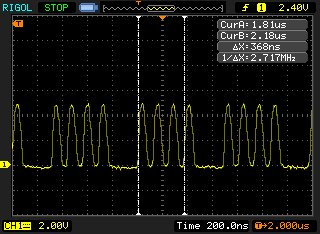
\includegraphics[width=0.45\textwidth]{../figs/speed-test-named-bits-inlined-pic18f26k22.jpeg}
  \end{center}
  With the bit-manipulation words \verb!RB1-hi! and \verb!RB1-lo! being
  inlined, they also achieve full machine speed because the generated code is essentially
  the same as for \verb!blink-asm!.
  % Incidentally, for this measurement, the oscilloscope lead had been switched to $10\times$ 
  % to reduce the capacitive loading on the MCU pin.
\end{itemize}


\subsection{PIC24FV32KA302}
%

\bigskip\noindent
\code{}{../pic24/speed-test-pic24fv32ka302.txt}

\noindent
Notes on this program:
\begin{itemize}
 \item The order of the assembler arguments is bit-number register-address op-code.
  This is different to that seen in the PIC18 version of the program.
 \item The MCU was configured for running off its internal 8\,MHz oscillator with
  the 4$\times$ PLL active and a 1:1 postscaling.  
  This resulted in an instruction cycle period $T_{CY} = 62.5$\,ns.
 \item The screen image on the left shows the output signal for running the high-level
  \verb!blink-forth! word while the image on the right uses the assembler words.
  \begin{center}
  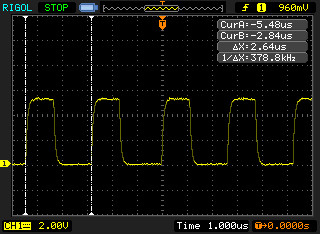
\includegraphics[width=0.45\textwidth]{../figs/speed-test-forth-pic24fv32ka302.jpeg}
  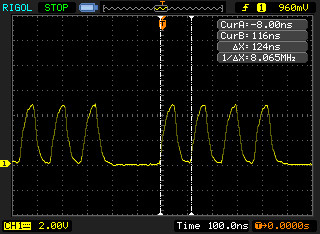
\includegraphics[width=0.45\textwidth]{../figs/speed-test-asm-pic24fv32ka302.jpeg}
  \end{center}
 \item For the \verb!blink-forth! word, one on+off cycle of the LED executes in 6 words
  and is seen (in the oscilloscope record) to require about 42 instruction cycles.
  So, on average, each of these threaded Forth words is executed by the 16-bit PIC24 in 7 MCU instruction cycles.
  This illustrates a benefit of the 16-bit processor, 
  since the 8-bit PIC18F26K22 required 50 MCU instruction cycles 
  (and a correspondingly longer time of 3.08\,microseconds) for the same effect.
 \item The assembler version has no overhead and the cycle time for the MCU
  instructions defines the period of the output signal.
  One on-off cycle requires 2 instructions so we see a short 124\,ns period.
 \item The oscilloscope record for the \verb!blink-bits! word is shown here.
  \begin{center}
  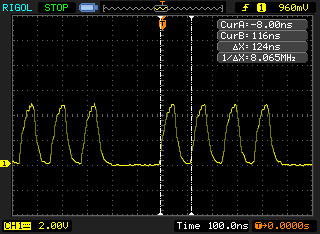
\includegraphics[width=0.45\textwidth]{../figs/speed-test-named-bits-inlined-pic24fv32ka302.jpeg}
  \end{center}
  Again, the bit-manipulation words \verb!RB15-hi! and \verb!RB15-lo! also achieve full machine speed.
\end{itemize}


\subsection{ATmega328P}
%

\bigskip\noindent
\code{}{../avr8-2016/speed-test.txt}

\noindent
Notes on this program:
\begin{itemize}
 \item Except for names, this code is essentially the same as for the PIC18 and PIC24
  versions of the exercise.  FlashForth abstracts away much of the instruction-set architecture
  of the microcontroller, leaving us to focus on twiddling the bits of the peripheral hardware.
 \item The MCU was configured for running with the 16\,MHz crystal,
  which resulted in a machine clock cycle period $T_{CY} = 62.5$\,ns.
 \item The screen image on the left shows the output signal for running the high-level
  \verb!blink-forth! word while the image on the right uses the assembler words.
  \begin{center}
  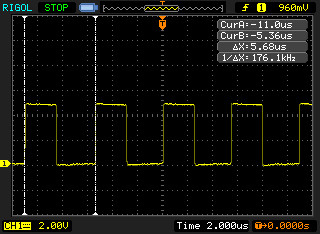
\includegraphics[width=0.45\textwidth]{../figs/speed-test-forth-atmega328-2016.jpeg}
  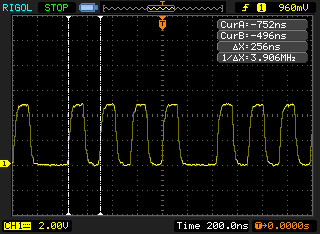
\includegraphics[width=0.45\textwidth]{../figs/speed-test-asm-atmega328-2016.jpeg}
  \end{center}
 \item For the \verb!blink-forth!, one on+off cycle of the LED executes in 6 words
  and is seen (in the oscilloscope record) to require about 90 instruction cycles.
  So, on average, each of these threaded Forth words is executed by the 8-bit AVR in 15 MCU instruction cycles. 
 \item The assembler version has no overhead and the cycle time for the MCU
  instructions defines the period of the output signal.
  One on-off cycle requires 2 instructions (\verb!sbi! and \verb!cbi!) each requiring 2 clock cycles,
  so we see a short, quarter-microsecond period.
 \item The oscilloscope record for the \verb!blink-bits! word is shown here.
  \begin{center}
  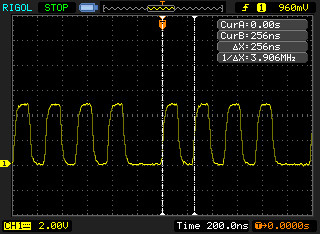
\includegraphics[width=0.45\textwidth]{../figs/speed-test-named-bits-inlined-atmega328-2016.jpeg}
  % 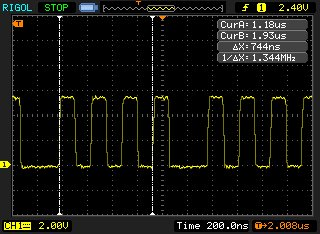
\includegraphics[width=0.45\textwidth]{../figs/speed-test-named-bits-io-inlined-atmega328.jpeg}
  \end{center}
  It can be seen that the bit-manipulation words \verb!PB5-hi! and \verb!PB5-lo! achieve full machine speed.
\end{itemize}


%\bigskip
\newpage
\section{Driving an Hitachi-44780 LCD controller}
\label{lcd-example-sec}
%
The LCD in the photograph on page\,\pageref{lcd-on-picdem2-board} was driven with the following code.
During the development of this example, a lesson was relearned -- that of reading 
the data sheet\,\cite{hitachi-hd44780-datasheet} carefully :)

\bigskip\noindent
\code{}{../pic18/xlcd.txt}

\newpage
\bibliographystyle{unsrt}
\bibliography{ff}

\appendix
\newpage
\section{Using other terminal programs}
\label{other-terminal-programs-sec}
%
As discussed in Section\,\ref{interacting-with-flashforth-sec},
interaction with the programmed MCU is via the serial port.
There are a number of generic terminal emulation programs that will
communicate via a serial port.
On a Linux machine the \texttt{cutecom} terminal program is very convenient.
It has a line-oriented input that doesn't send the text to the MCU until
you press the enter key.
This allows for editing of the line before committing it to the MCU and
convenient recall of previous lines.
\texttt{GtkTerm} is available as more conventional terminal program.
The following images shows the GtkTerm window just after sending the content
of the \verb!flash-led.txt! file to the PIC18F26K22.
The device name of \verb!/dev/ttyUSB0! refers to the USB-to-serial interface 
that was plugged one of the PC's USB ports.
It is convenient to start GtkTerm with the command
\begin{verbatim}
$ sudo gtkterm 
\end{verbatim}
and then adjust the communication settings via the \verb!Configuration! $\rightarrow$ \verb!Port! menu item 
and its associated dialog window.

\medskip
\noindent
\begin{center}
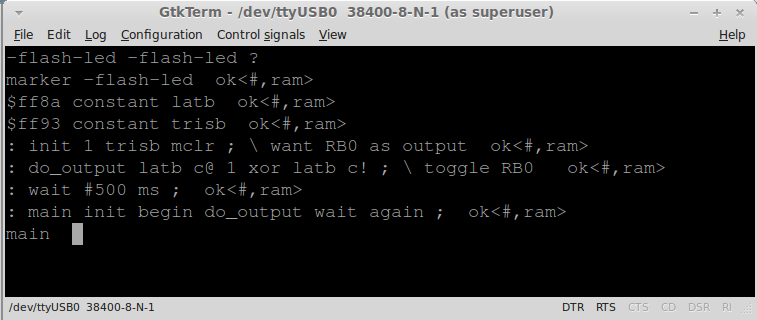
\includegraphics[width=0.7\textwidth]{../figs/gtkterm-with-FF5p0-flash-led-pic18.png}
\end{center}

\medskip\noindent
There is also a send-file capability and, importantly, the capability to
set the period between lines of text that are sent to the serial port 
so as to not overwhelm the FlashForth MCU.
Although USB-to-serial interfaces usually implement software Xon-Xoff
handshaking, my experience of using them with a minimal 3-wire connection 
(GND, RX and TX) has been variable.
When sending large files, an end-of-line delay of a few tens of milliseconds 
has usually been found adequate, however, there have been times that a file 
would not successfully load until the end-of-line pause was increased to 300\,milliseconds.
For \verb!GtkTerm!, this setting is under the \verb!Advanced Configuration Options! 
in the port configuration dialog, as shown below.
This end-of-line delay makes the transfer of large files slow, however,
the text still scrolls past quickly but is now at a pace where it is possible to follow 
the dialog and know how well the compilation is going.
Building your application code incrementally, with small files, is a good thing.

\medskip
\noindent
\begin{center}
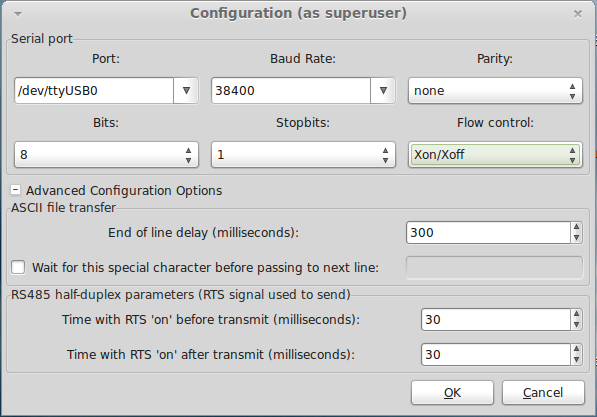
\includegraphics[width=0.5\textwidth]{../figs/gtkterm-configuration-dialog.png}
\end{center}

\medskip\noindent
For MacOSX, Thomas Buschhardt reports that \verb!CoolTerm! is a good choice for a terminal application.
It is available from \verb!http://freeware.the-meiers.org/!.

\medskip
\noindent
\begin{center}
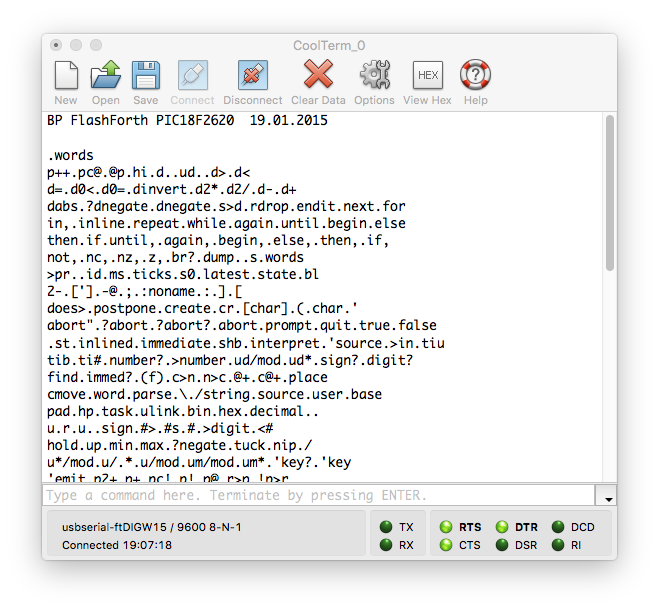
\includegraphics[width=0.5\textwidth]{../figs/coolterm.png}
\end{center}

\end{document}
